\documentclass[12pt, a4]{article}
\usepackage[english]{babel}
\usepackage[utf8]{inputenc}
\usepackage{fullpage}
\usepackage{listings}
\usepackage{graphicx}
\usepackage{color}

%Syntax highlighting
\definecolor{blue-violet}{rgb}{0.54, 0.17, 0.89}
\definecolor{ao}{rgb}{0.0, 0.5, 0.0}
\definecolor{amaranth}{rgb}{0.9, 0.17, 0.31}
\definecolor{ballblue}{rgb}{0.13, 0.67, 0.8}
\definecolor{onyx}{rgb}{0.06, 0.06, 0.06}


\lstset{
  breaklines=true,                 % automatic line breaking only at whitespace
  captionpos=b,                    % sets the caption-position to bottom
  breakatwhitespace=false,
  keepspaces=true,
  numbers=left,
  numbersep=5pt,
  showspaces=false,
  showstringspaces=false,
  showtabs=false,
  tabsize=4,  
  backgroundcolor=\color{white},   % choose the background color
  commentstyle=\color{ao},    % comment style
  keywordstyle=\color{amaranth},    % keyword style
  stringstyle=\color{blue-violet},    % string literal style
  numberstyle=\tiny\color{ballblue},	   % number style
  basicstyle=\ttfamily\footnotesize\color{onyx} % size of fonts used for the code
}


%Document Header
\title{\textbf{Department of CSE\\SSN College of Engineering}}
\author{\textbf{Vishakan Subramanian - 18 5001 196 - Semester VI}}
\date{30 March 2021}

\begin{document}
\maketitle
\hrule
\section*{\center{UCS 1611 - Internet Programming Lab}}
\hrule
\bigskip

%Assignment Details
\subsection*{\center{\textbf{Exercise 4: Java Servlets and MySQL}}}
\subsection*{\flushleft{Learning Objective:}}
\begin{flushleft}
Create a HTML file with following form fields:

\begin{enumerate}
\item Employee ID
\item Employee Name
\item Designation
\item Department
\item Basic Salary
\item Phone Number
\item Address
\item Date of Birth
\item Gender
\item Marital Status
\item Submit (Button, onclick submit the form details to a servlet)
\item Reset (Button, onclick)
\end{enumerate}

Write a servlet program which reads all form details, finds the gross pay based on basic pay and designation. The servlet returns all details (a-j, gross pay) in table format to the client.\newline 

Develop a Patient Management System (PMS) in a Hospital that maintains the
patient records, with the following specifications:

\begin{enumerate}
\item Admin only can access the patient records.
\item Admin has to authenticate himself with the credentials to access the
patient details.
\item The first page is the login page (login.html) where the admin should
enter the credentials.
\item If login fails, display an alert “Login Failed, enter the correct details”, clear the username and password textbox and focus the control back
to the username of login.html.
\item Perform the authentication using JavaScript, use hardcoded username
and password in login.html.
\item On successful login, it should be redirected to homepage
(homepage.html) of PMS.
\item The homepage.html should display the following: Add Record, Update Record, Delete Record, View Record \& Search Record.
\item Clicking the links should invoke its corresponding html file from where
the information is submitted to the corresponding Servlet.
\item When “View” button is clicked it invokes the “ViewServlet” to display all
the records in the database.
\item Similarly, perform ADD, UPDATE, VIEW and SEARCH using corresponding
html and Servlet.
\item UPDATE is invoked if phone number or Address of the patient is
changed.
\item SEARCH for particular patient based on Patient ID.
\item After each operation ViewServlet should be invoked to view the changes
in the Database.
\end{enumerate}

Database Name: Patient$\_$Details\\
Table Schema: Name, Age, ID, Gender, Address, Phone Number, Marital status, Date of Visit.
 
\end{flushleft}

%Code
\newpage
\subsection*{\flushleft{Code - Employee Registration Page HTML:}}
\begin{flushleft}
\lstinputlisting[language = HTML]{employee/index.html}
\end{flushleft}

\newpage
\subsection*{\flushleft{Code - Employee Registration Page CSS:}}
\begin{flushleft}
\lstinputlisting[language = HTML]{employee/styles.css}
\end{flushleft}

\newpage
\subsection*{\flushleft{Code - Web XML:}}
\begin{flushleft}
\lstinputlisting[language = XML]{employee/WEB-INF/web.xml}
\end{flushleft}

\newpage
\subsection*{\flushleft{Code - Employee Servlet:}}
\begin{flushleft}
\lstinputlisting[language = Java]{employee/Form.java}
\end{flushleft}

%Output
\newpage
\subsection*{\flushleft{Output - Employee Registration Page:}}
\begin{figure}[h]
\centering
\caption{Browser Output: Employee Registration Page.}
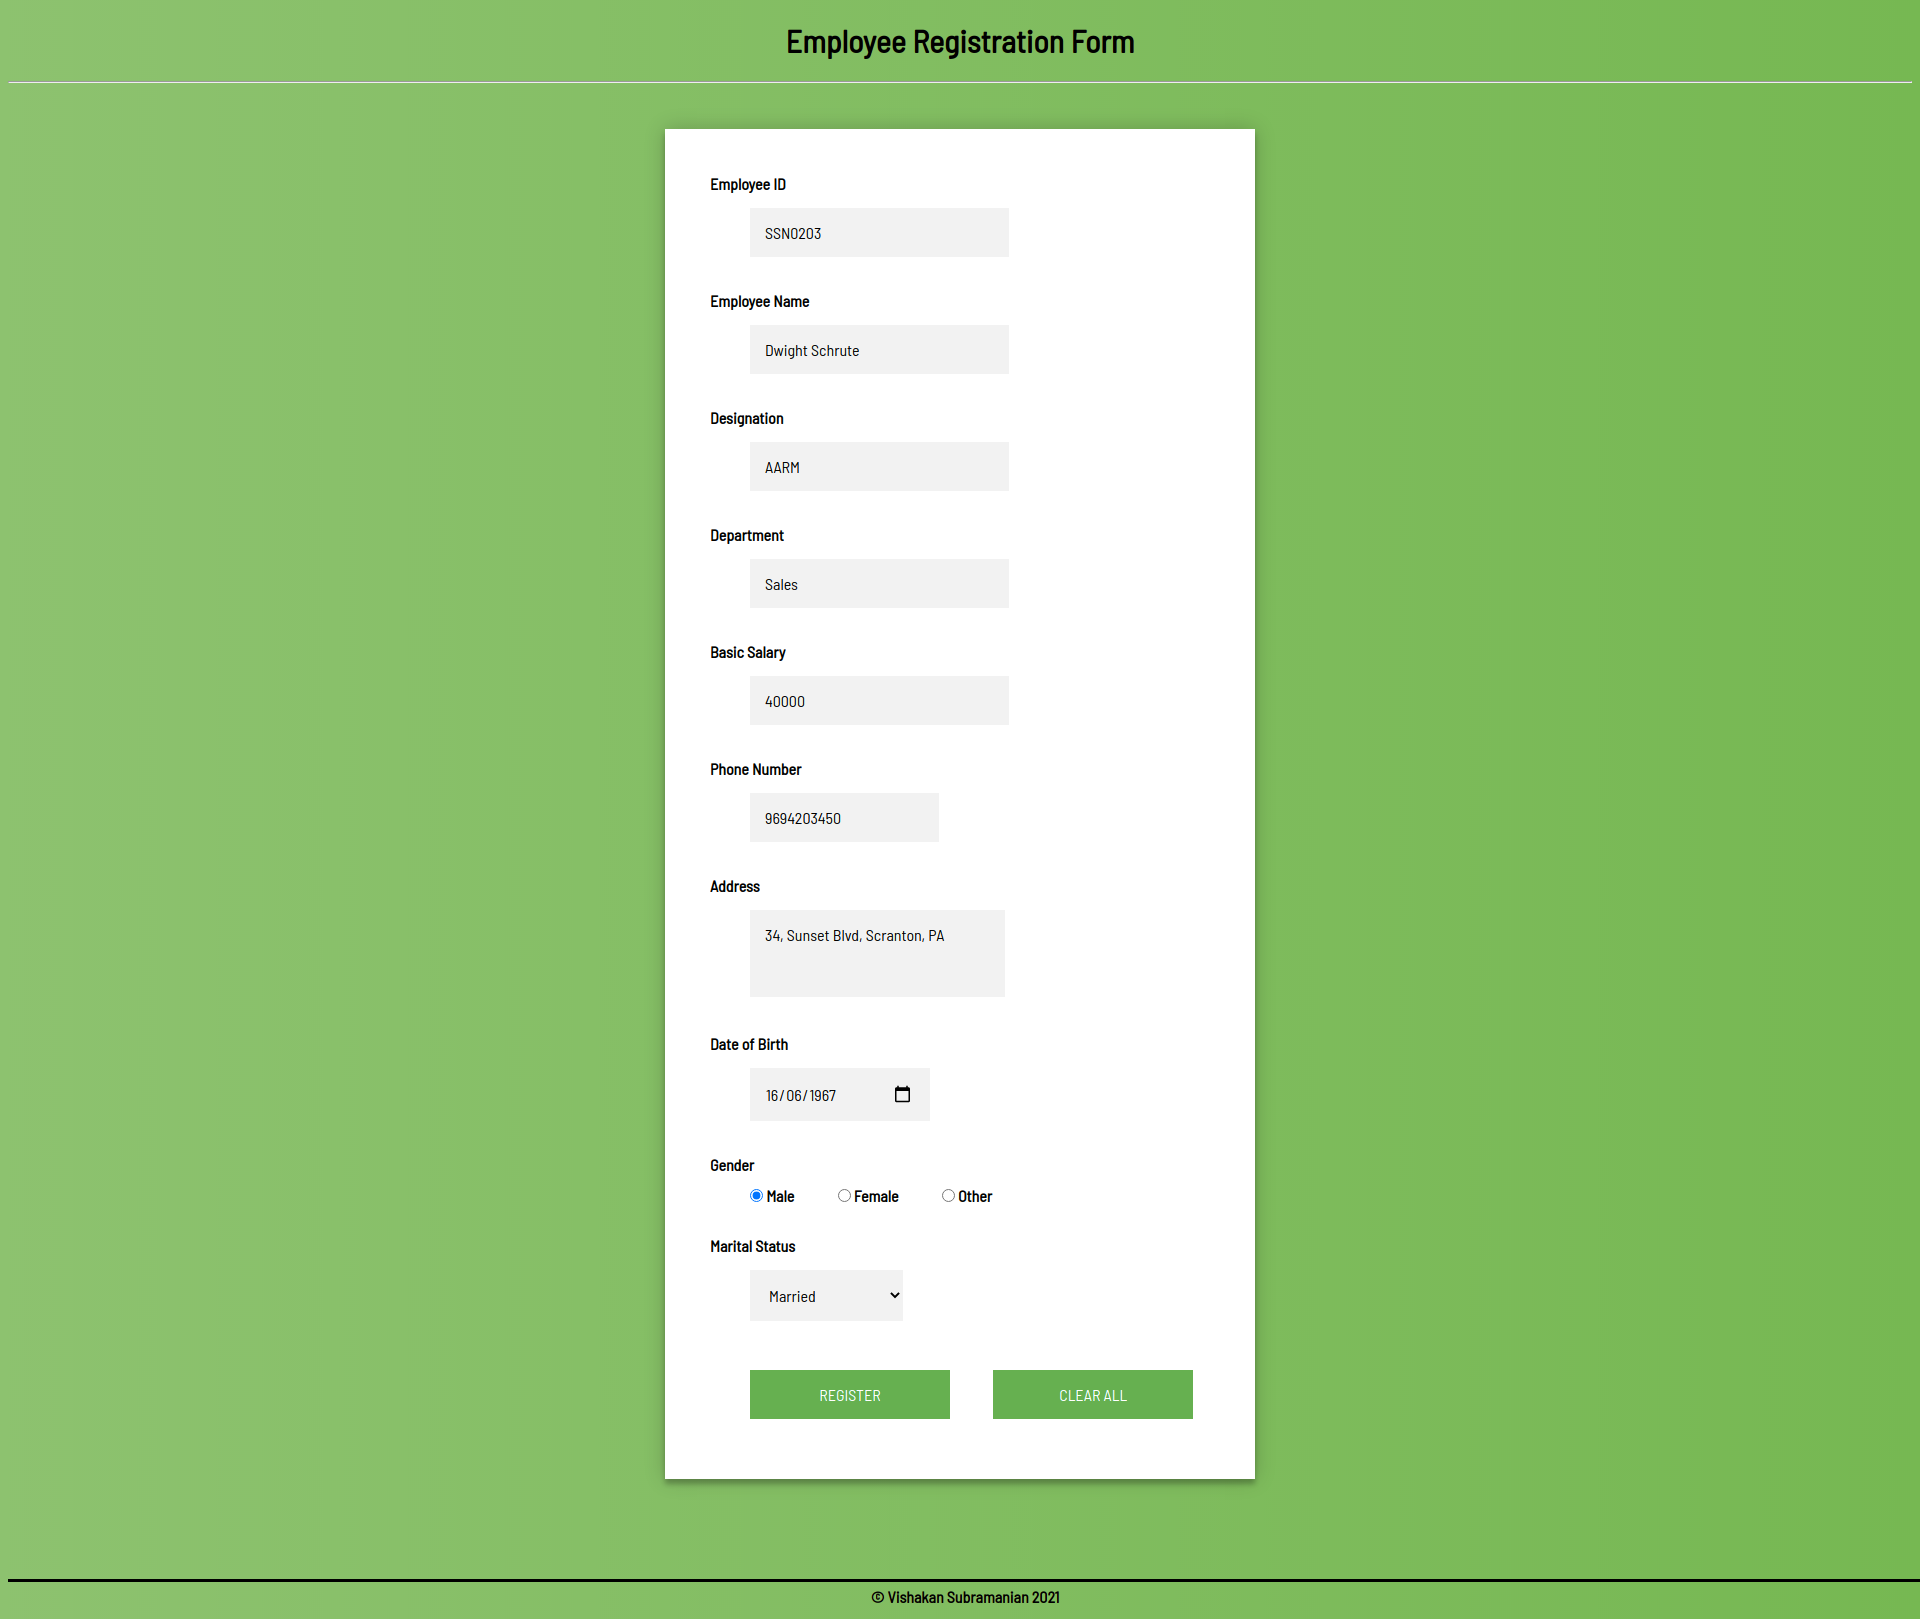
\includegraphics[height=15cm, width=18cm]{Output/Employee1.png}
\end{figure}

\newpage
\subsection*{\flushleft{Output - Employee Servlet Page:}}
\begin{figure}[h]
\centering
\caption{Browser Output: Employee Servlet Page.}
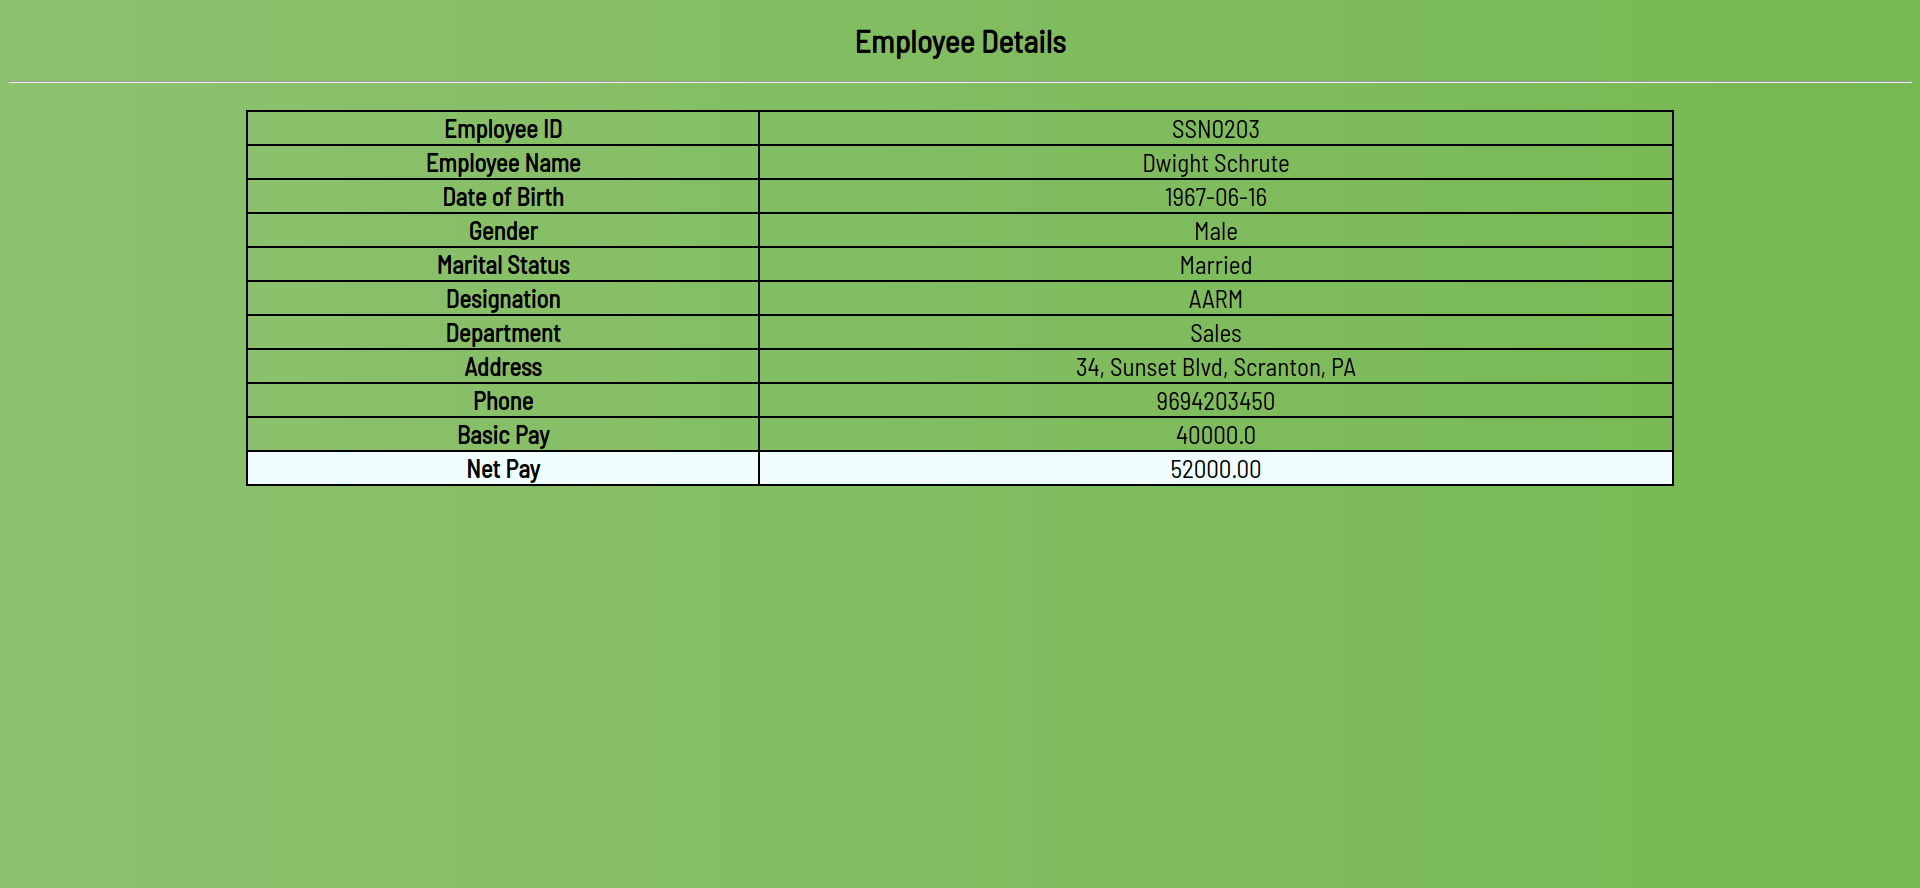
\includegraphics[height=12cm, width=18cm]{Output/Employee2.png}
\end{figure}

\newpage
\subsection*{\flushleft{Code - Login Page HTML:}}
\begin{flushleft}
\lstinputlisting[language = HTML]{pms/login.html}
\end{flushleft}

\newpage
\subsection*{\flushleft{Code - Home Page HTML:}}
\begin{flushleft}
\lstinputlisting[language = HTML]{pms/homepage.html}
\end{flushleft}

\newpage
\subsection*{\flushleft{Code - Add Record Page HTML:}}
\begin{flushleft}
\lstinputlisting[language = HTML]{pms/add.html}
\end{flushleft}

\newpage
\subsection*{\flushleft{Code - Update Record Page HTML:}}
\begin{flushleft}
\lstinputlisting[language = HTML]{pms/update.html}
\end{flushleft}

\newpage
\subsection*{\flushleft{Code - Delete Record Page HTML:}}
\begin{flushleft}
\lstinputlisting[language = HTML]{pms/delete.html}
\end{flushleft}

\newpage
\subsection*{\flushleft{Code - View Records Page HTML:}}
\begin{flushleft}
\lstinputlisting[language = HTML]{pms/view.html}
\end{flushleft}

\newpage
\subsection*{\flushleft{Code - Search Records Page HTML:}}
\begin{flushleft}
\lstinputlisting[language = HTML]{pms/search.html}
\end{flushleft}

\newpage
\subsection*{\flushleft{Code - Pages CSS:}}
\begin{flushleft}
\lstinputlisting[language = HTML]{pms/css/pages.css}
\end{flushleft}

\newpage
\subsection*{\flushleft{Code - Script JS:}}
\begin{flushleft}
\lstinputlisting[language = HTML]{pms/scripts/login.js}
\end{flushleft}

\newpage
\subsection*{\flushleft{Code - Script SQL:}}
\begin{flushleft}
\lstinputlisting[language = SQL]{pms/scripts/script.sql}
\end{flushleft}


\newpage
\subsection*{\flushleft{Code - Web XML:}}
\begin{flushleft}
\lstinputlisting[language = XML]{pms/WEB-INF/web.xml}
\end{flushleft}

\newpage
\subsection*{\flushleft{Code - Add Record Servlet:}}
\begin{flushleft}
\lstinputlisting[language = Java]{pms/Servlets/AddRecord.java}
\end{flushleft}

\newpage
\subsection*{\flushleft{Code - Update Record Servlet:}}
\begin{flushleft}
\lstinputlisting[language = Java]{pms/Servlets/UpdateRecord.java}
\end{flushleft}

\newpage
\subsection*{\flushleft{Code - Delete Record Servlet:}}
\begin{flushleft}
\lstinputlisting[language = Java]{pms/Servlets/DeleteRecord.java}
\end{flushleft}

\newpage
\subsection*{\flushleft{Code - Search Record Servlet:}}
\begin{flushleft}
\lstinputlisting[language = Java]{pms/Servlets/SearchRecord.java}
\end{flushleft}

\newpage
\subsection*{\flushleft{Code - View Records Servlet:}}
\begin{flushleft}
\lstinputlisting[language = Java]{pms/Servlets/ViewRecords.java}
\end{flushleft}

%Output
\newpage
\subsection*{\flushleft{Output - PMS Login Page:}}
\begin{figure}[h]
\centering
\caption{Browser Output: PMS Login Page.}
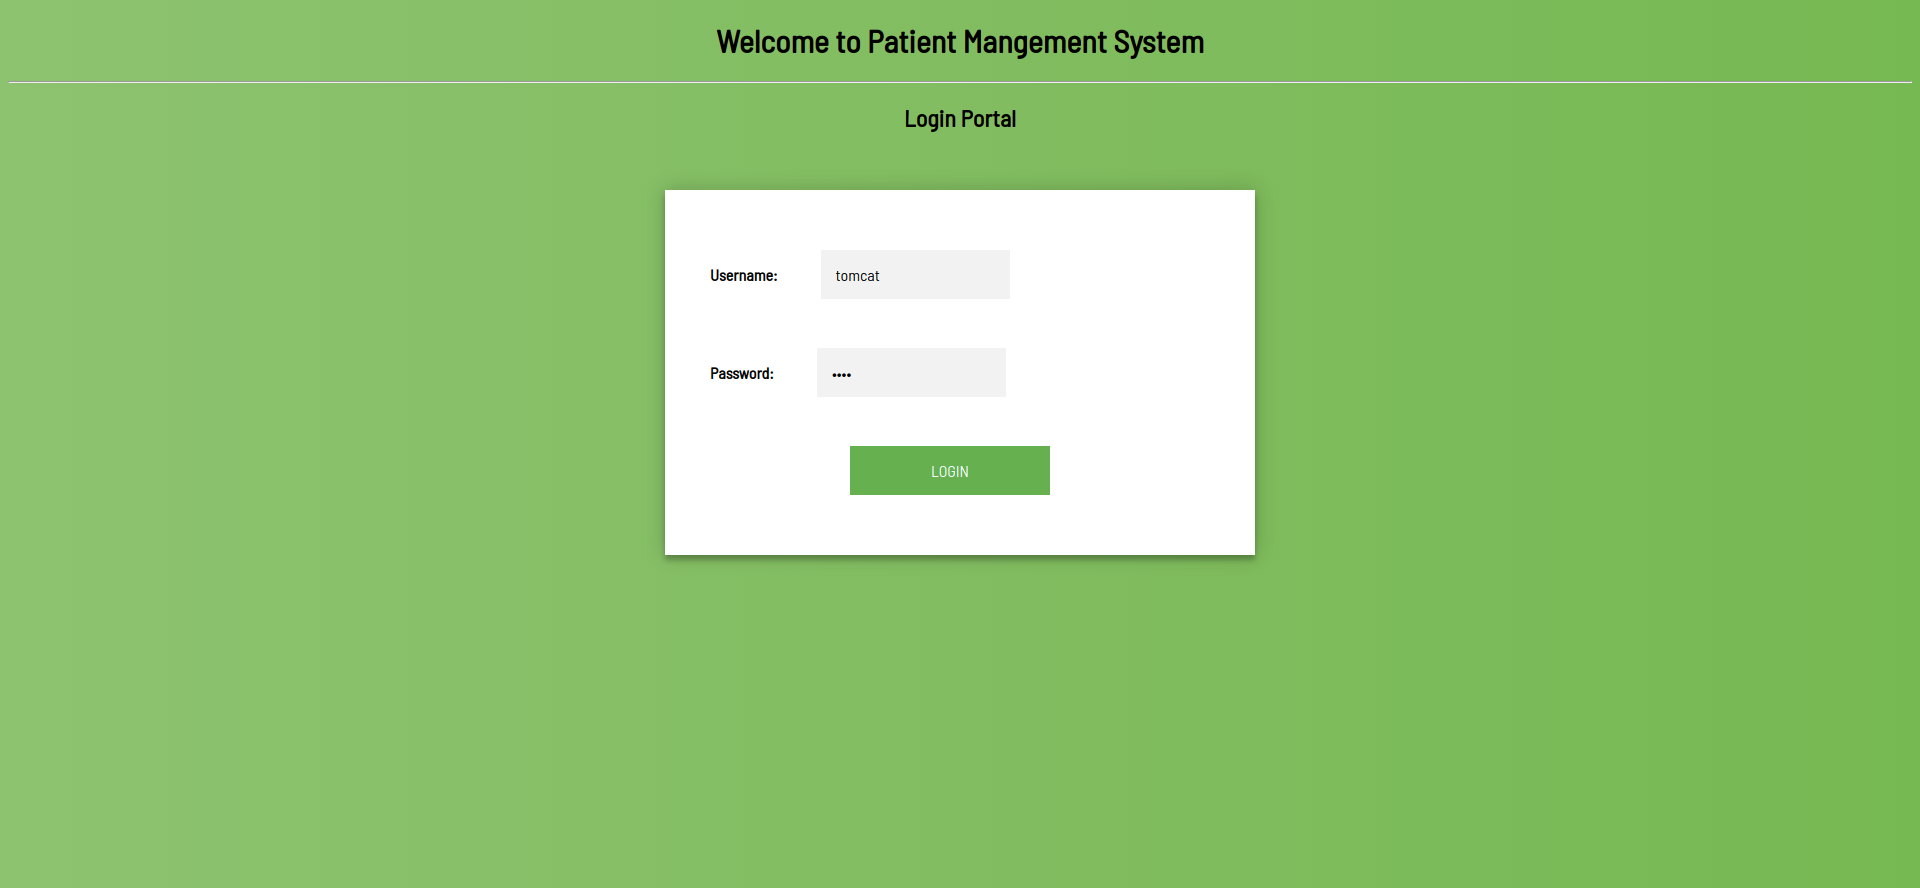
\includegraphics[height=12cm, width=16cm]{Output/PMSLogin.png}
\end{figure}

\newpage
\subsection*{\flushleft{Output - PMS Home Page:}}
\begin{figure}[h]
\centering
\caption{Browser Output: PMS Home Page.}
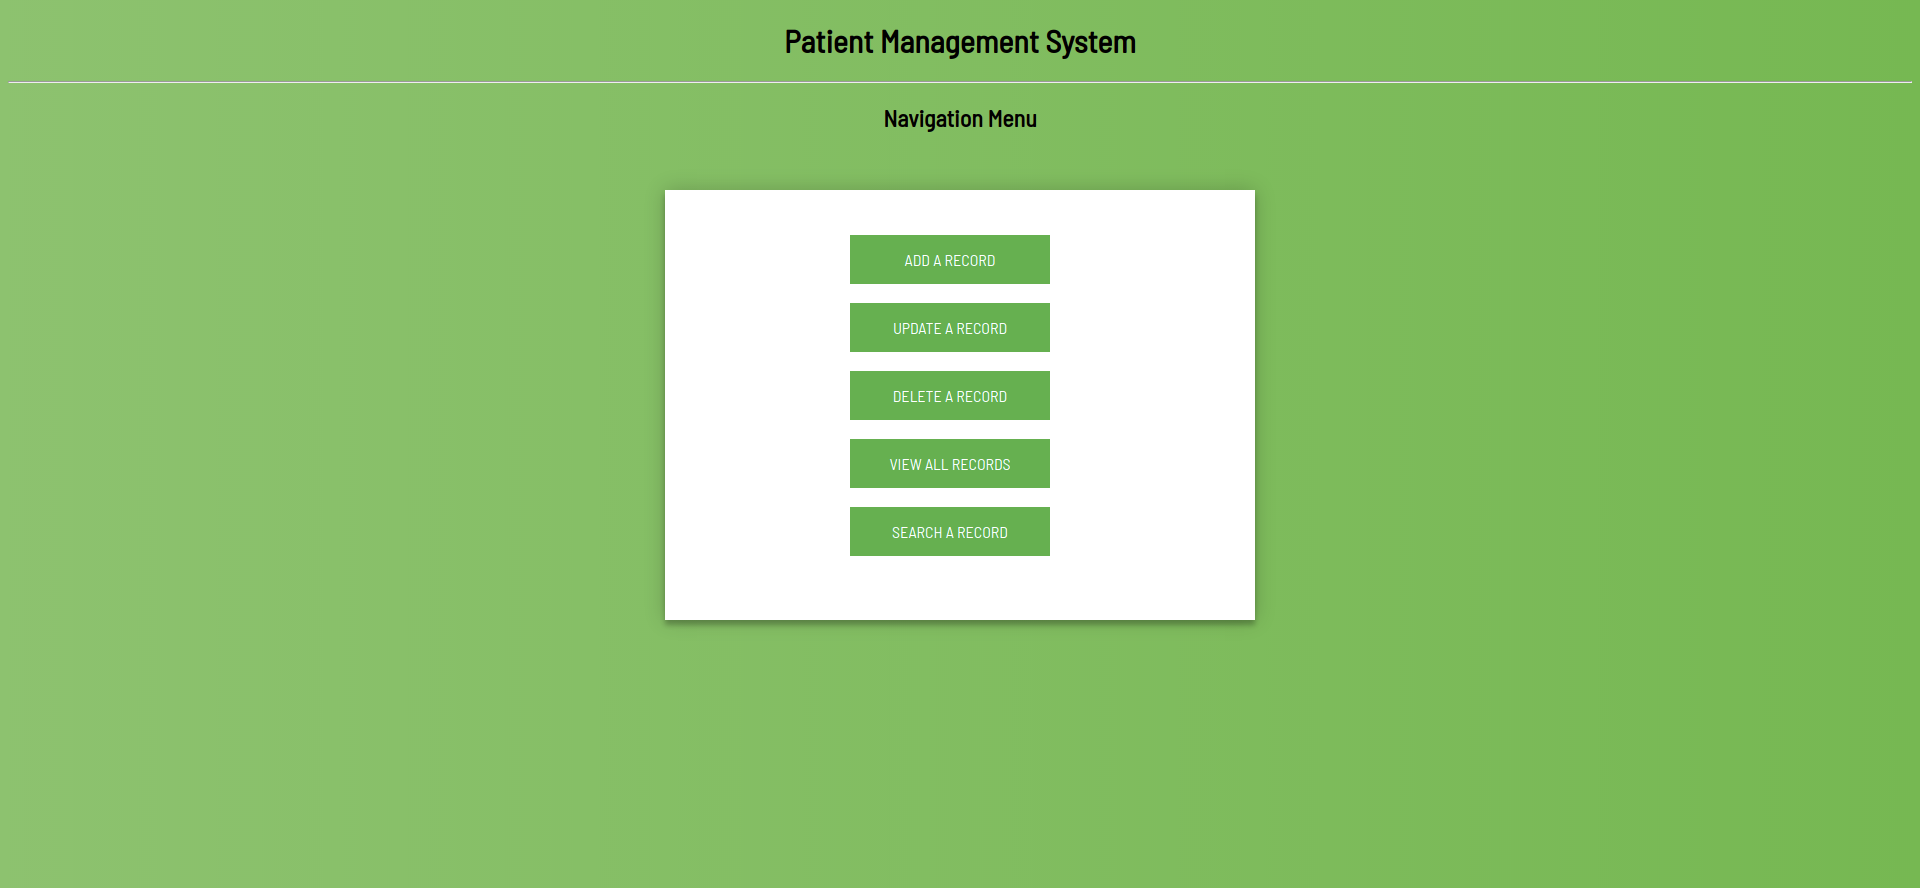
\includegraphics[height=12cm, width=16cm]{Output/PMSMenu.png}
\end{figure}

\newpage
\subsection*{\flushleft{Output - PMS Add Record Page:}}
\begin{figure}[h]
\centering
\caption{Browser Output: PMS Add Record Page.}
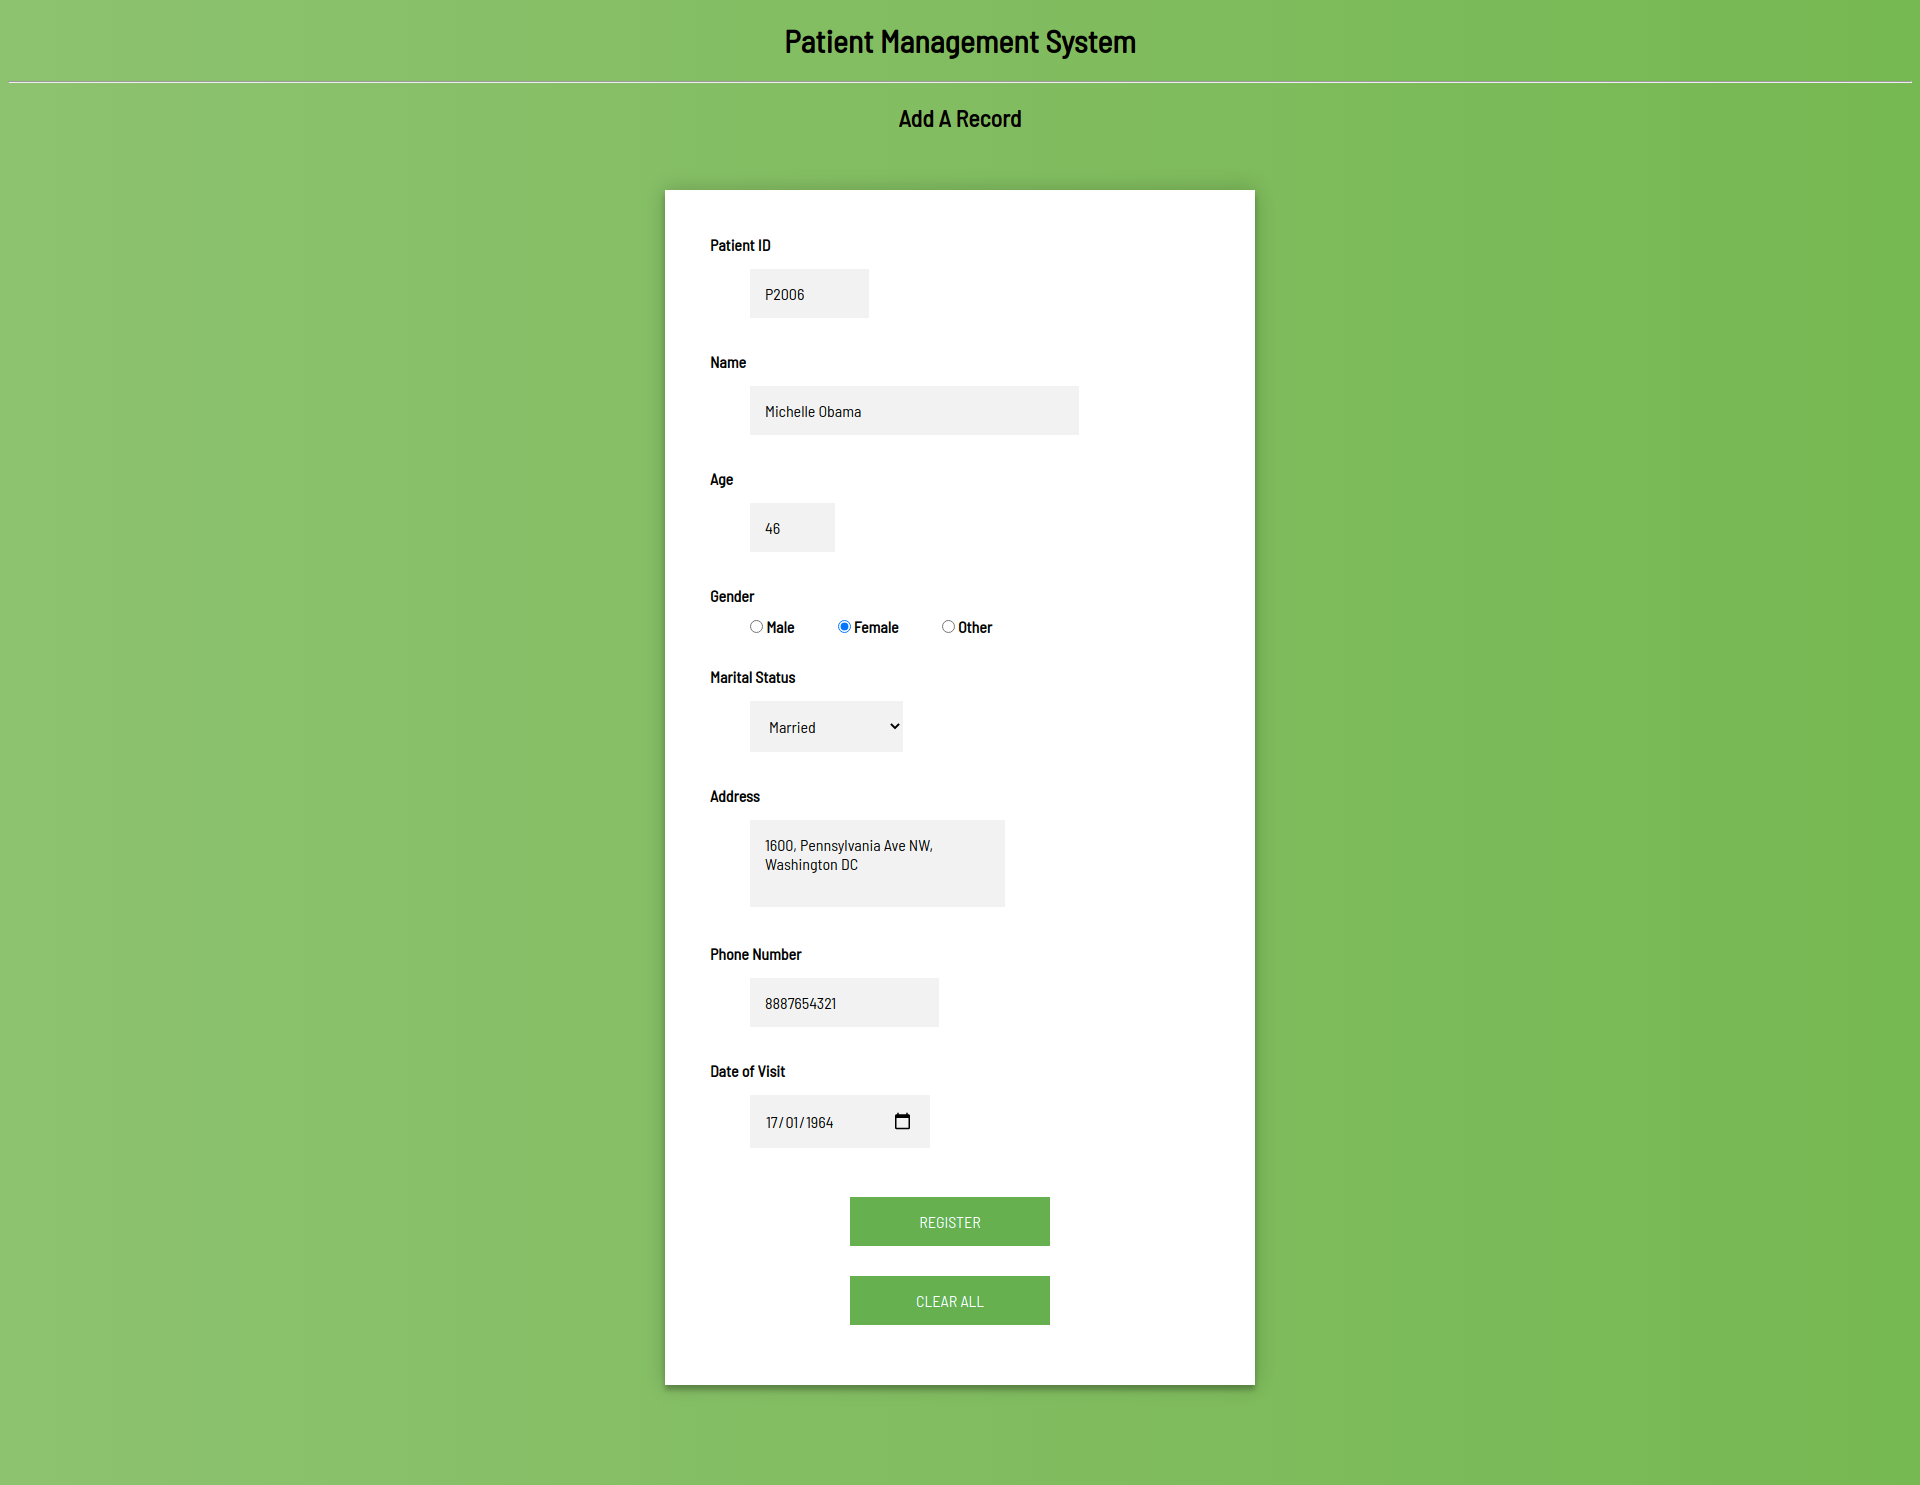
\includegraphics[height=15cm, width=18cm]{Output/PMSAdd.png}
\end{figure}

\newpage
\subsection*{\flushleft{Output - PMS Add Success Page:}}
\begin{figure}[h]
\centering
\caption{Browser Output: PMS Add Record Success Page.}
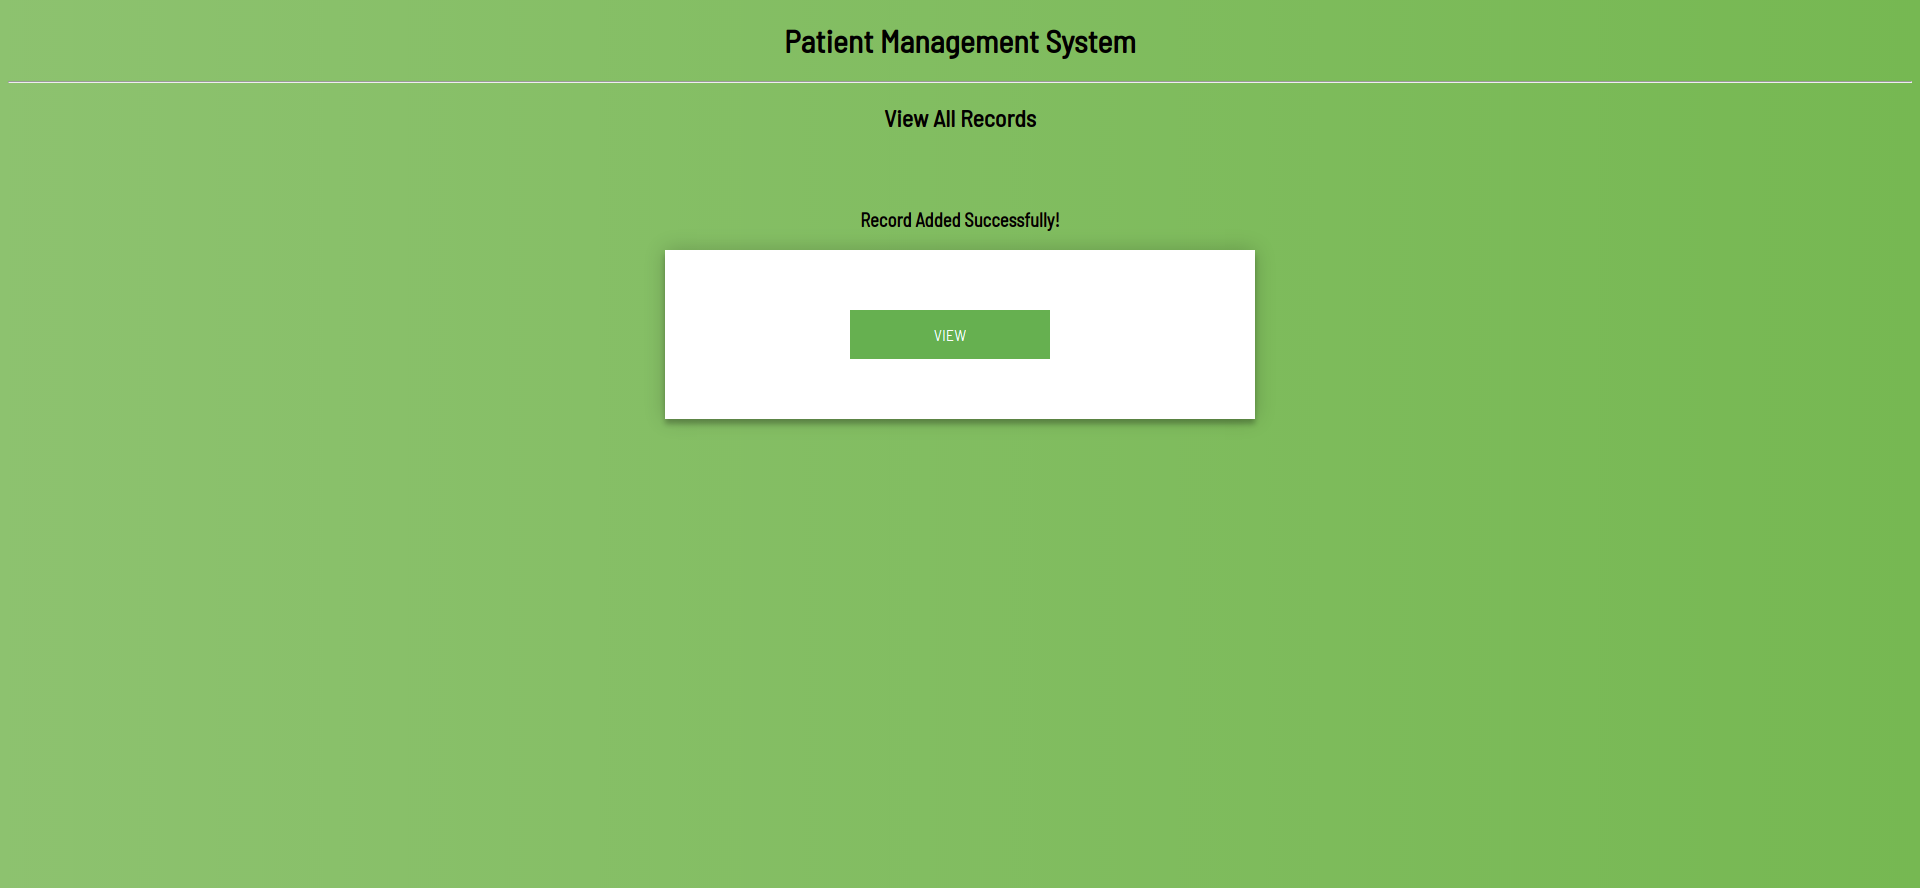
\includegraphics[height=12cm, width=16cm]{Output/PMSAddDone.png}
\end{figure}

\newpage
\subsection*{\flushleft{Output - PMS View Page:}}
\begin{figure}[h]
\centering
\caption{Browser Output: PMS View Page.}
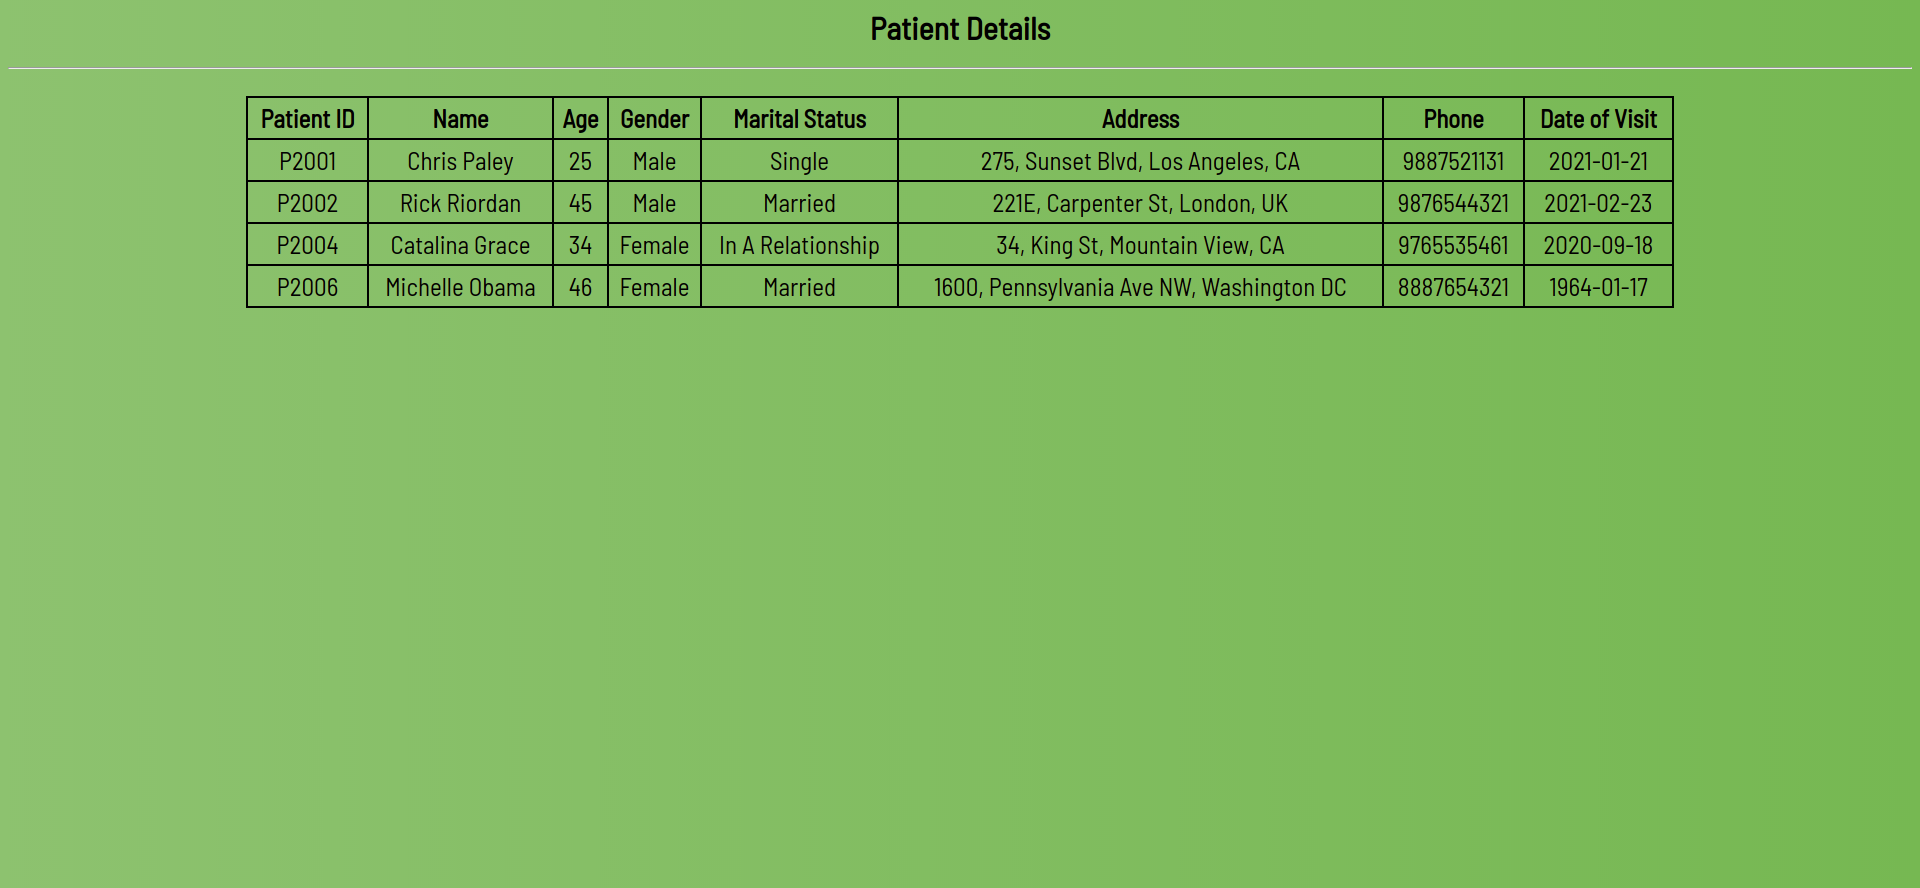
\includegraphics[height=12cm, width=16cm]{Output/PMSView1.png}
\end{figure}

\newpage
\subsection*{\flushleft{Output - PMS Update Record Page:}}
\begin{figure}[h]
\centering
\caption{Browser Output: PMS Update Record Page.}
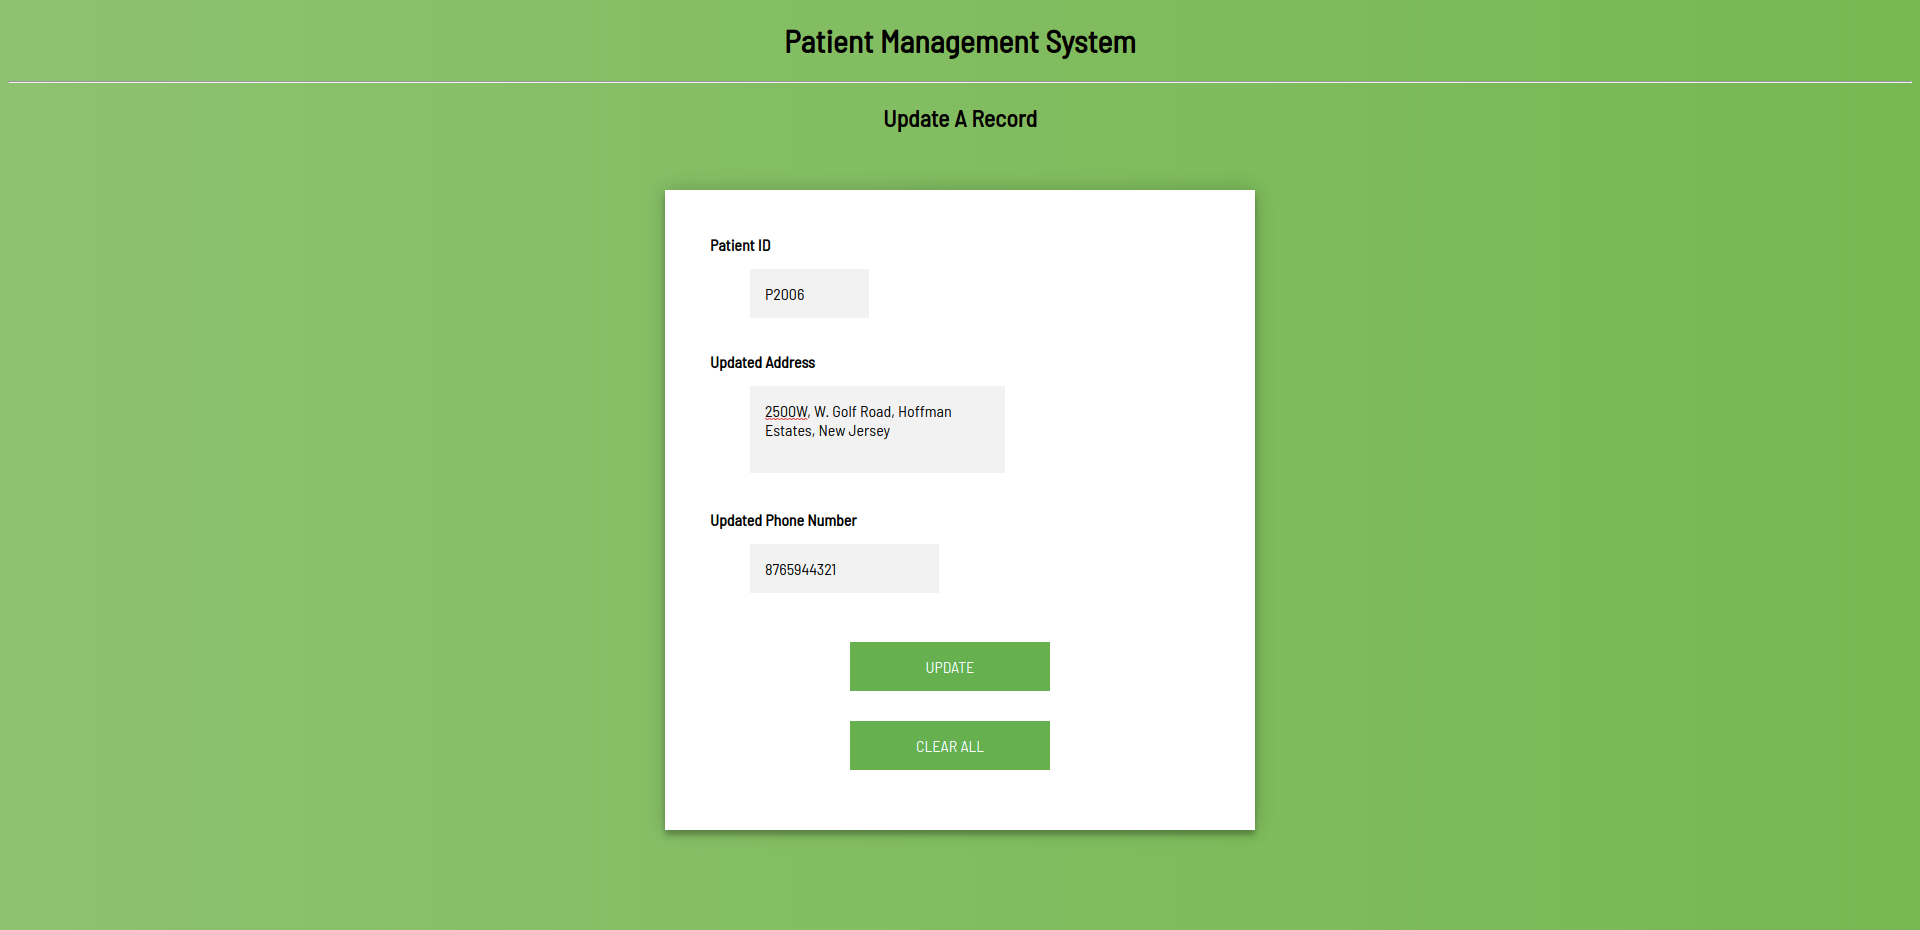
\includegraphics[height=12cm, width=18cm]{Output/PMSUpdate.png}
\end{figure}

\newpage
\subsection*{\flushleft{Output - PMS Update Success Page:}}
\begin{figure}[h]
\centering
\caption{Browser Output: PMS Update Record Success Page.}
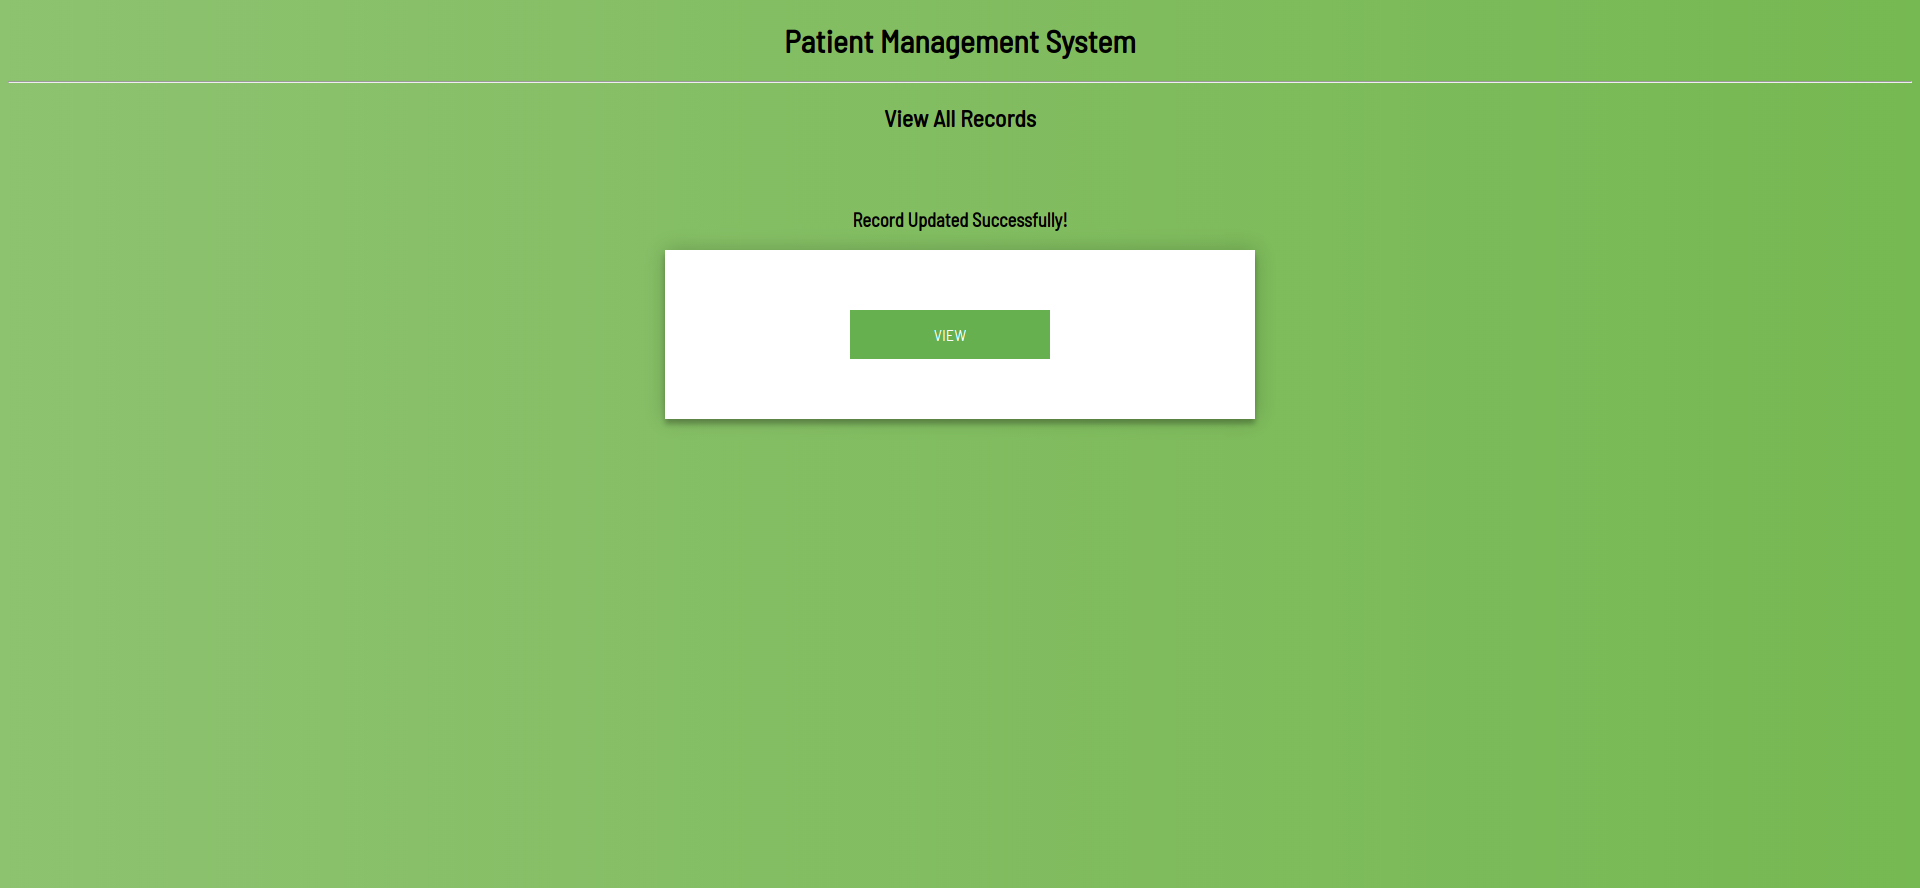
\includegraphics[height=12cm, width=16cm]{Output/PMSUpdateDone.png}
\end{figure}

\newpage
\subsection*{\flushleft{Output - PMS View Page:}}
\begin{figure}[h]
\centering
\caption{Browser Output: PMS View Page.}
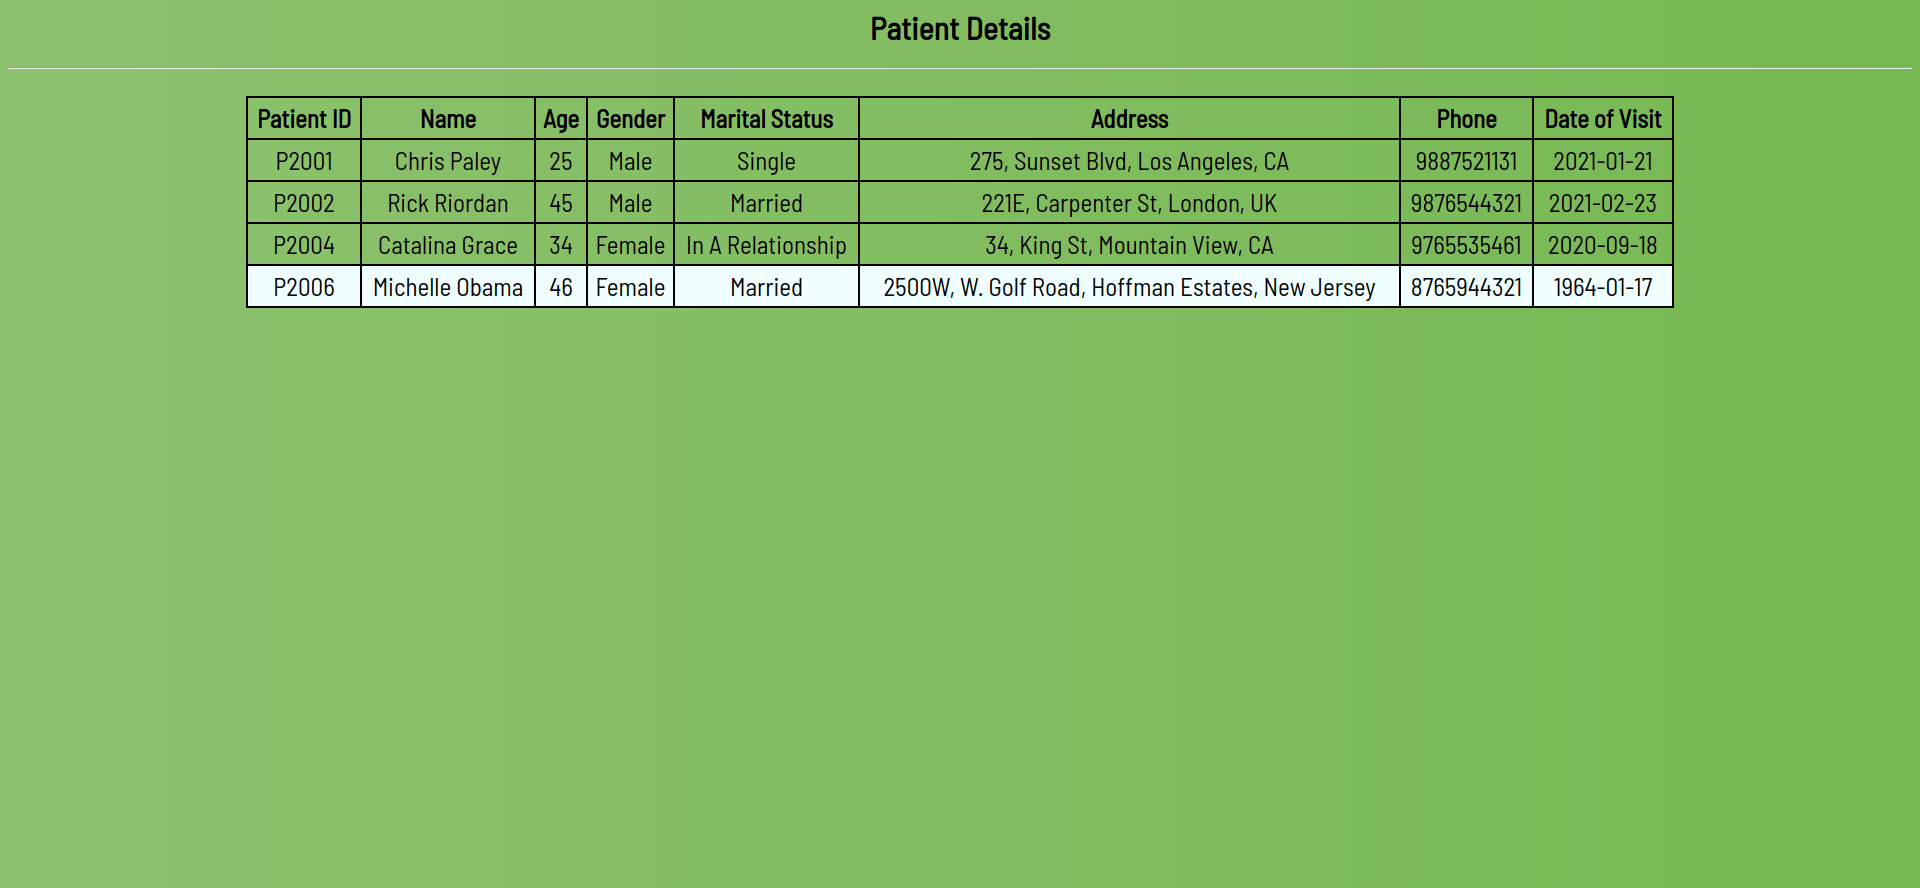
\includegraphics[height=12cm, width=16cm]{Output/PMSView2.png}
\end{figure}

\newpage
\subsection*{\flushleft{Output - PMS Delete Record Page:}}
\begin{figure}[h]
\centering
\caption{Browser Output: PMS Delete Record Page.}
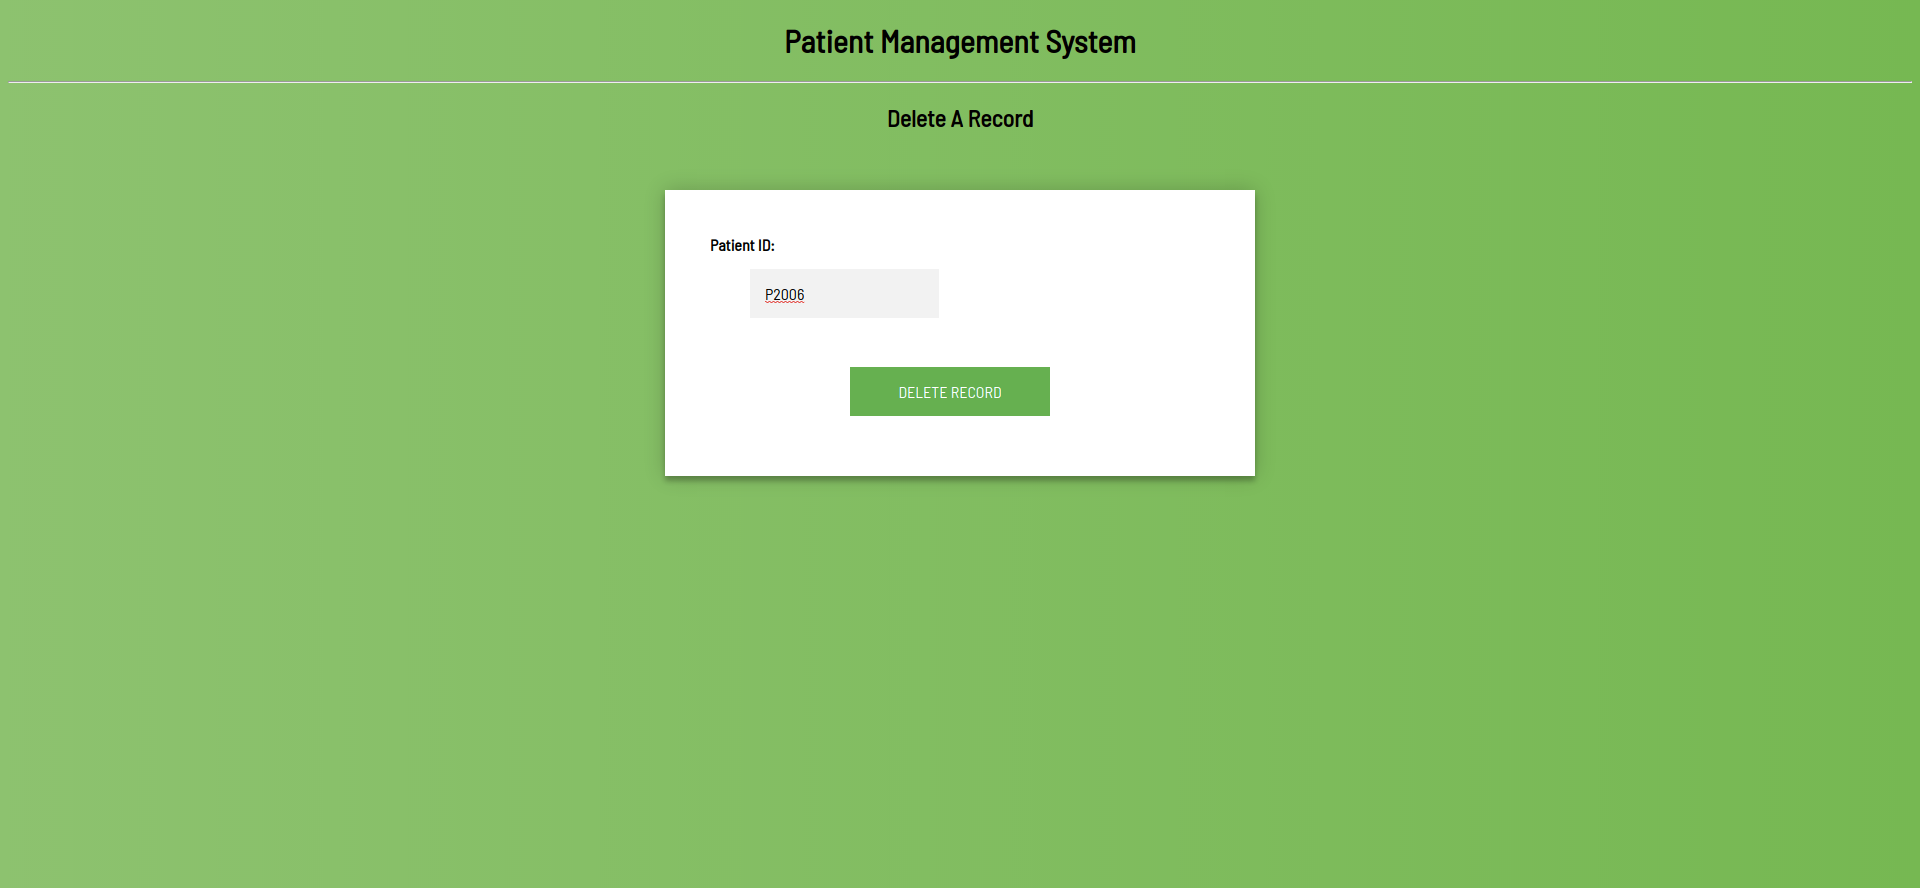
\includegraphics[height=12cm, width=16cm]{Output/PMSDelete.png}
\end{figure}

\newpage
\subsection*{\flushleft{Output - PMS Delete Success Page:}}
\begin{figure}[h]
\centering
\caption{Browser Output: PMS Delete Record Success Page.}
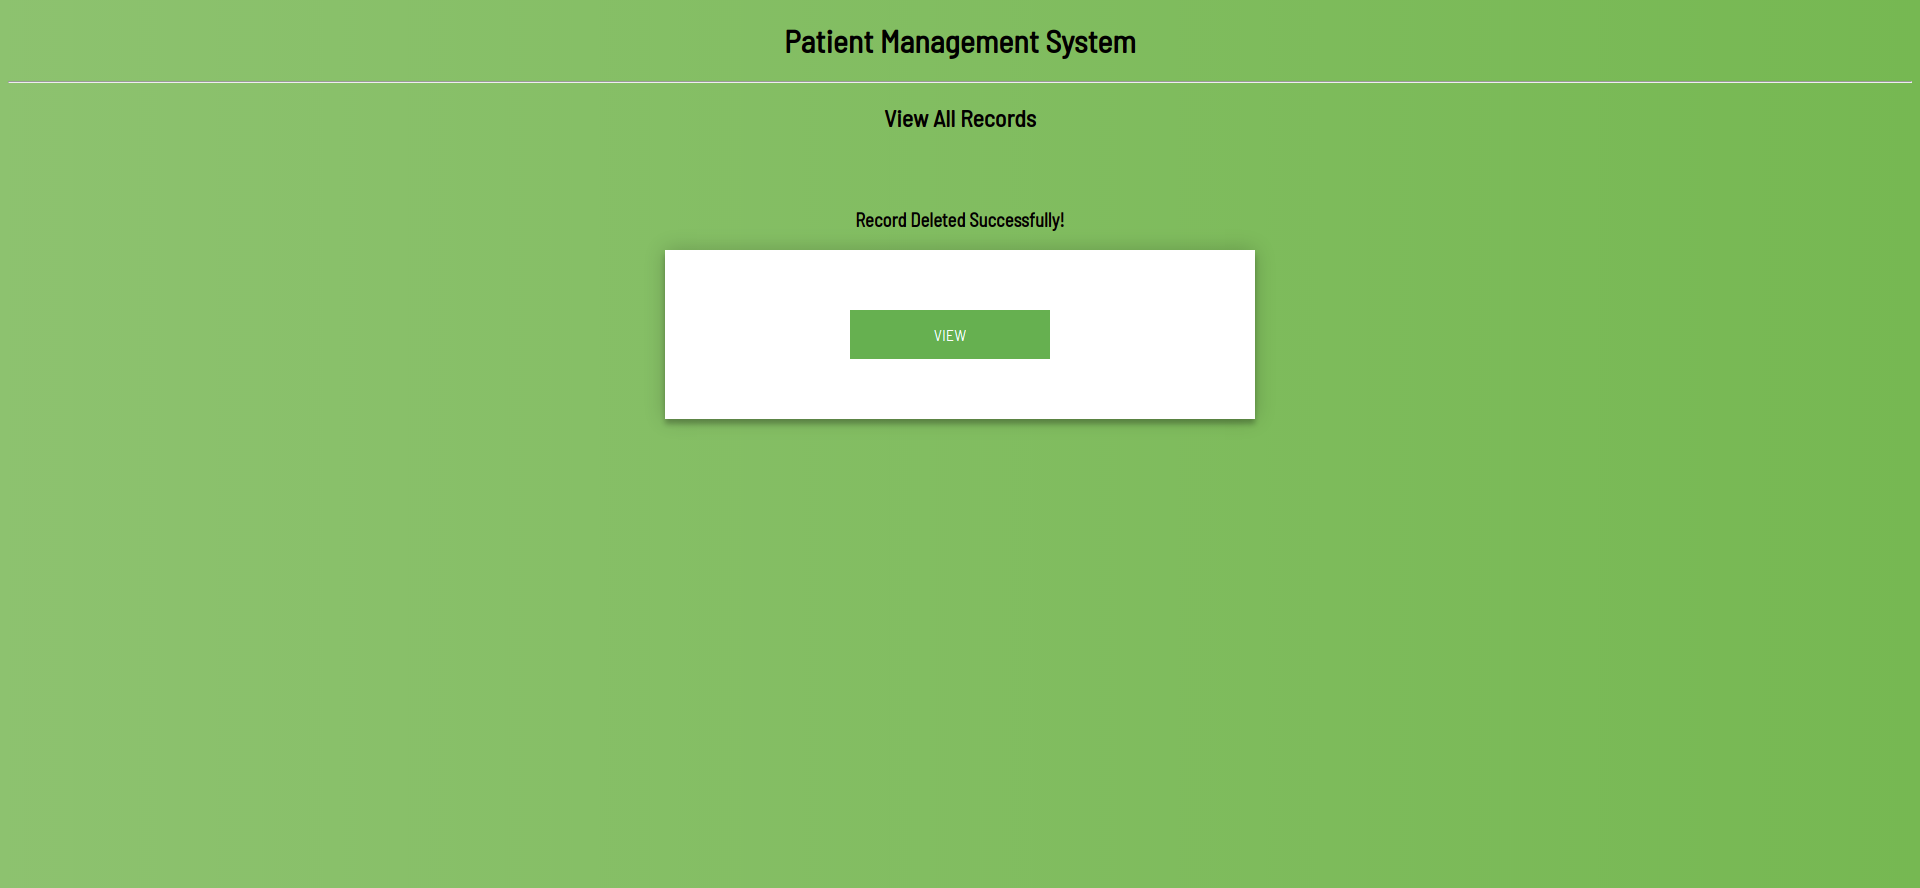
\includegraphics[height=12cm, width=16cm]{Output/PMSDeleteDone.png}
\end{figure}

\newpage
\subsection*{\flushleft{Output - PMS View Page:}}
\begin{figure}[h]
\centering
\caption{Browser Output: PMS View Page.}
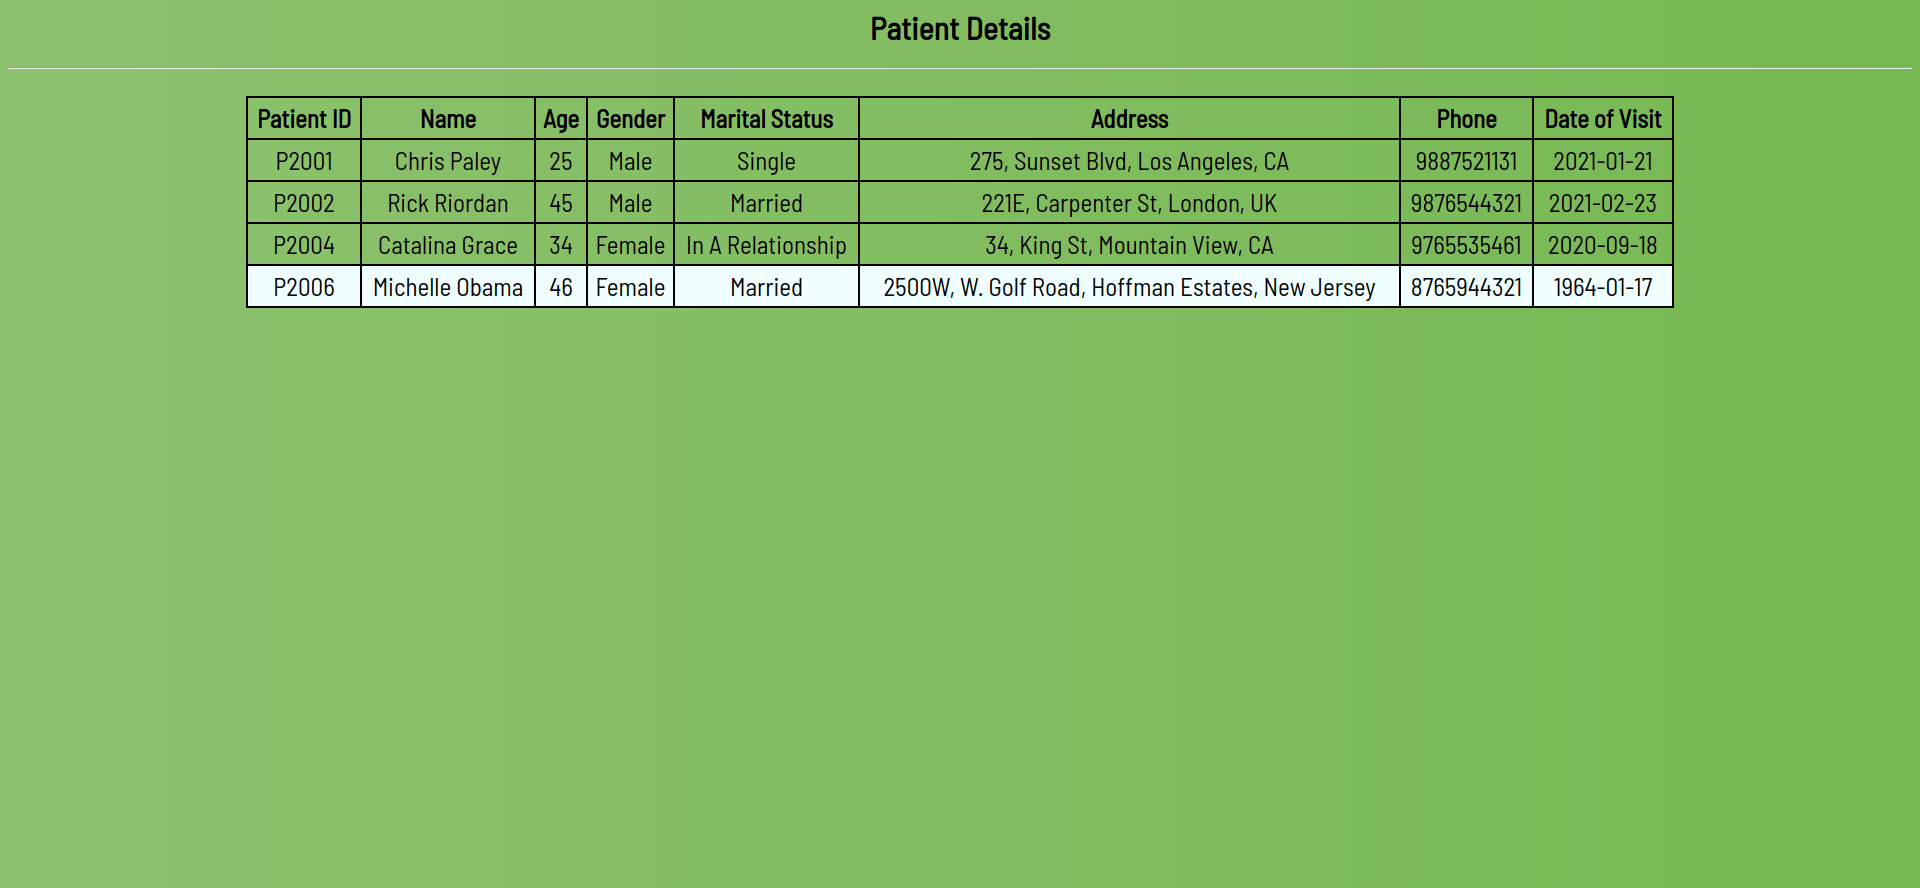
\includegraphics[height=12cm, width=16cm]{Output/PMSView2.png}
\end{figure}

\newpage
\subsection*{\flushleft{Output - PMS View Records Page:}}
\begin{figure}[h]
\centering
\caption{Browser Output: PMS View Records Page.}
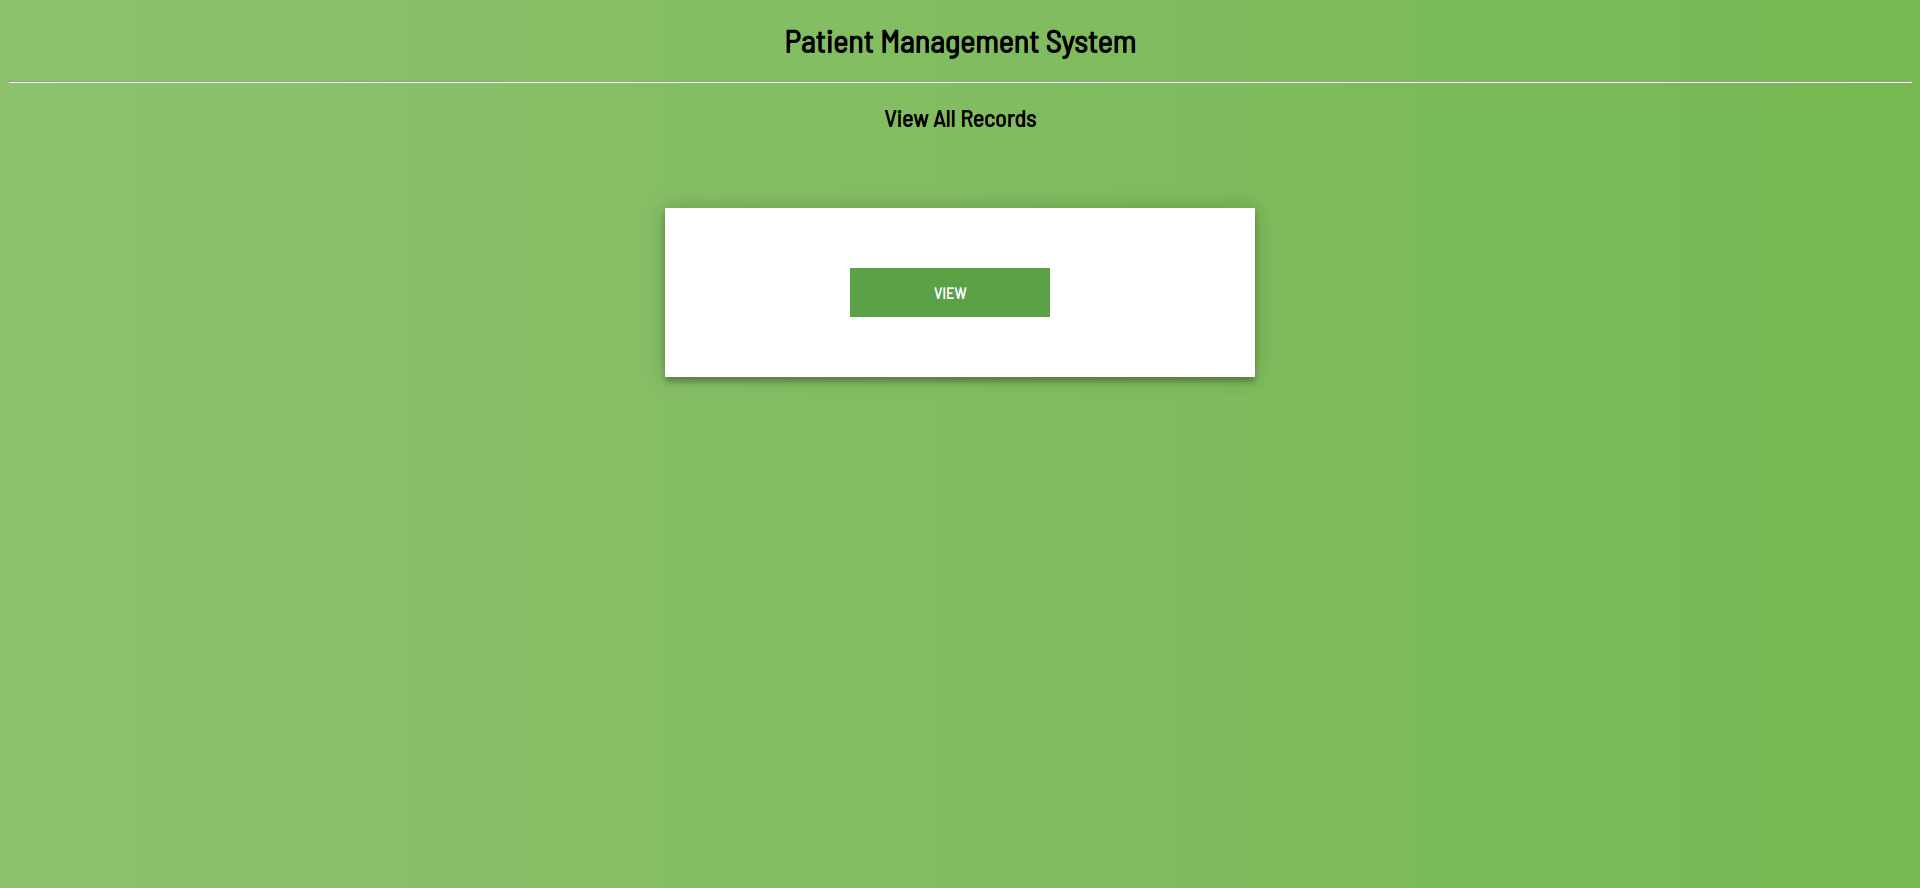
\includegraphics[height=12cm, width=16cm]{Output/PMSView0.png}
\end{figure}

\newpage
\subsection*{\flushleft{Output - PMS View Table Page:}}
\begin{figure}[h]
\centering
\caption{Browser Output: PMS View Table Page.}
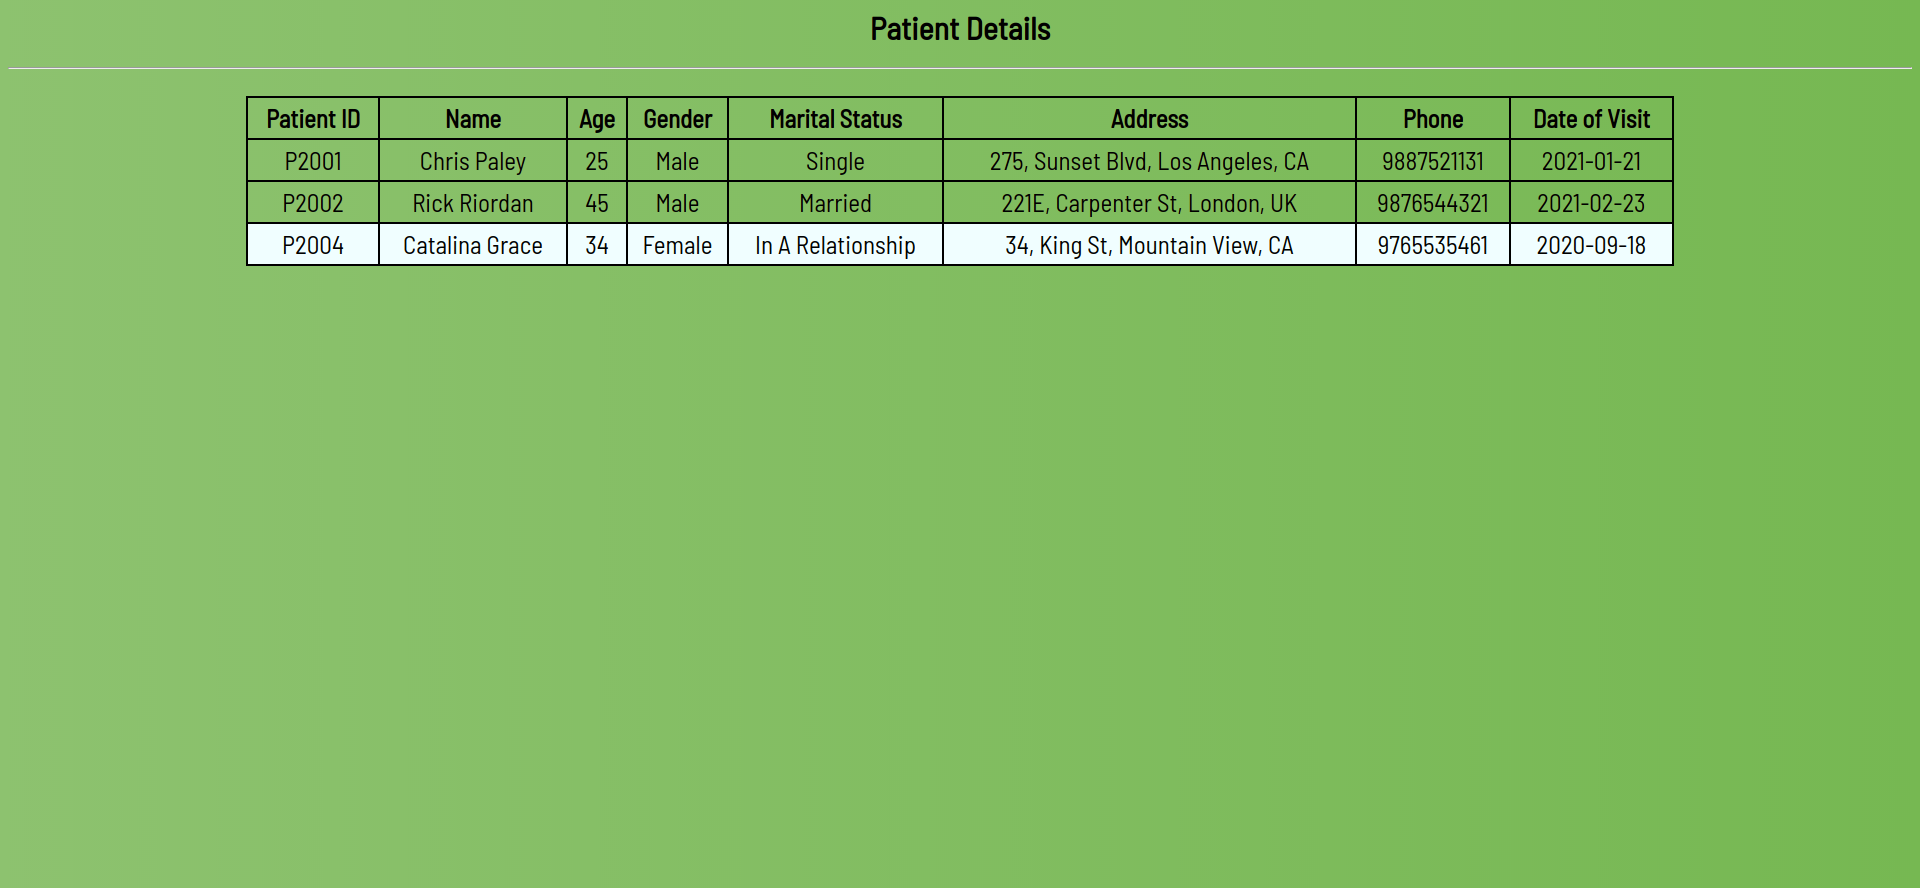
\includegraphics[height=12cm, width=16cm]{Output/PMSView3.png}
\end{figure}

\newpage
\subsection*{\flushleft{Output - PMS Search Record Page:}}
\begin{figure}[h]
\centering
\caption{Browser Output: PMS Search Record Page.}
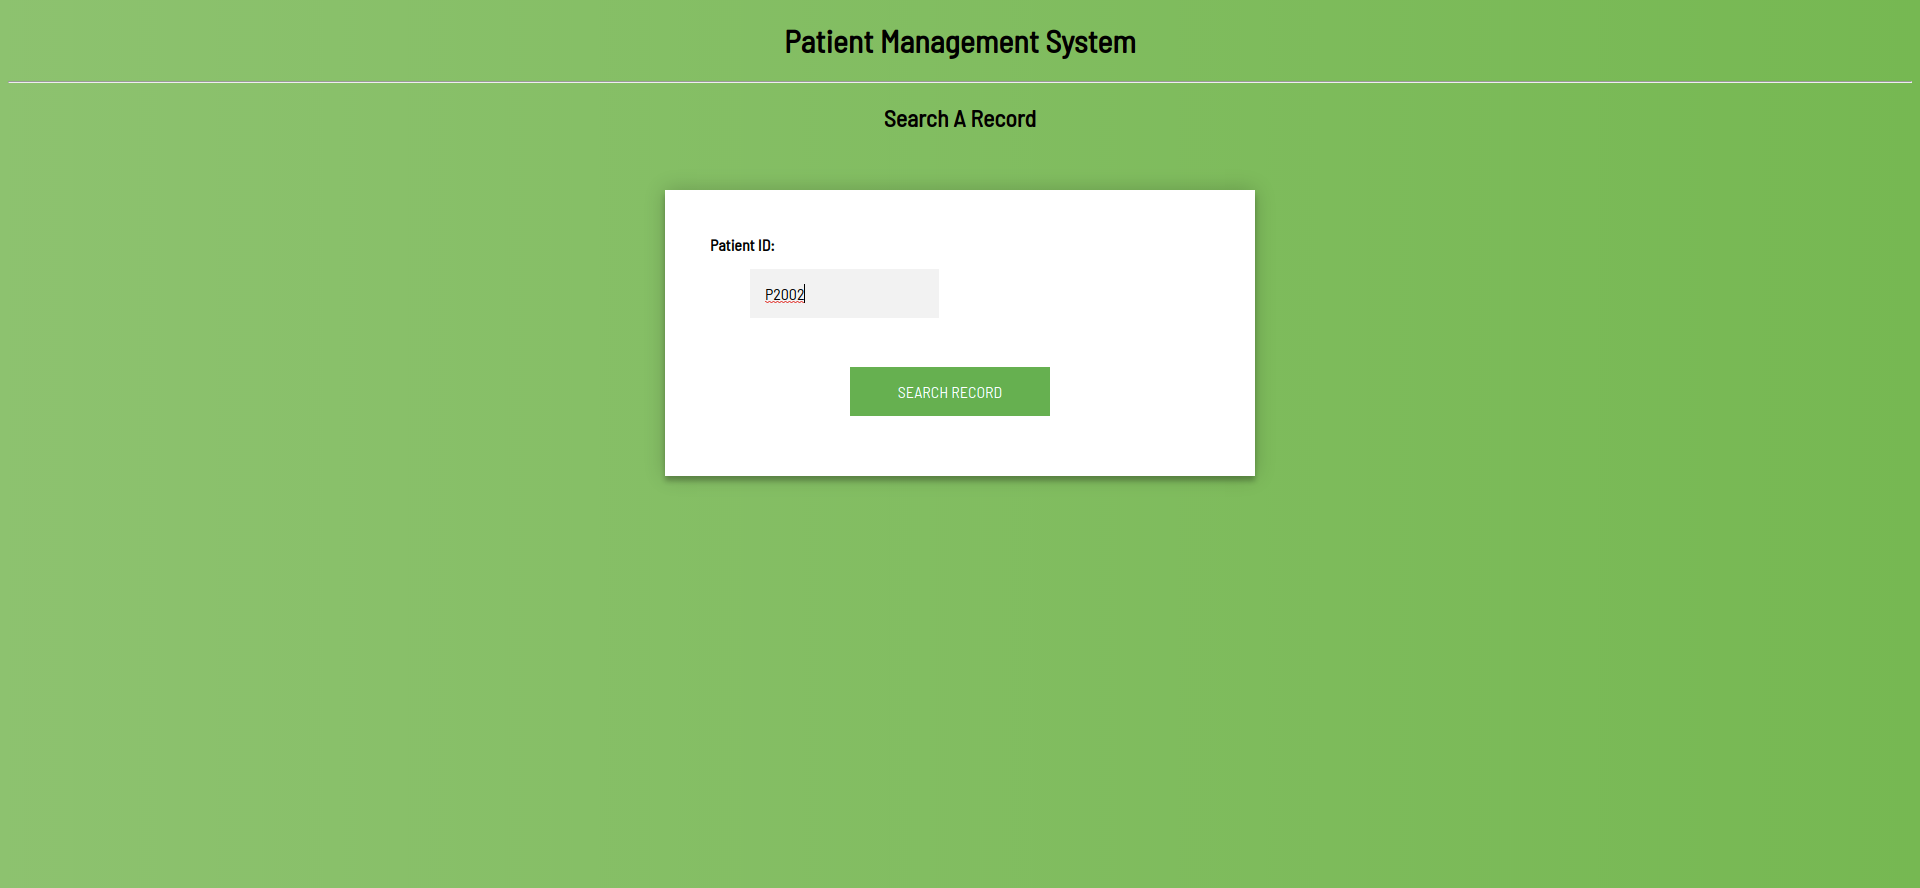
\includegraphics[height=12cm, width=16cm]{Output/PMSSearch.png}
\end{figure}

\newpage
\subsection*{\flushleft{Output - PMS Search Success Page:}}
\begin{figure}[h]
\centering
\caption{Browser Output: PMS Search Record Success Page.}
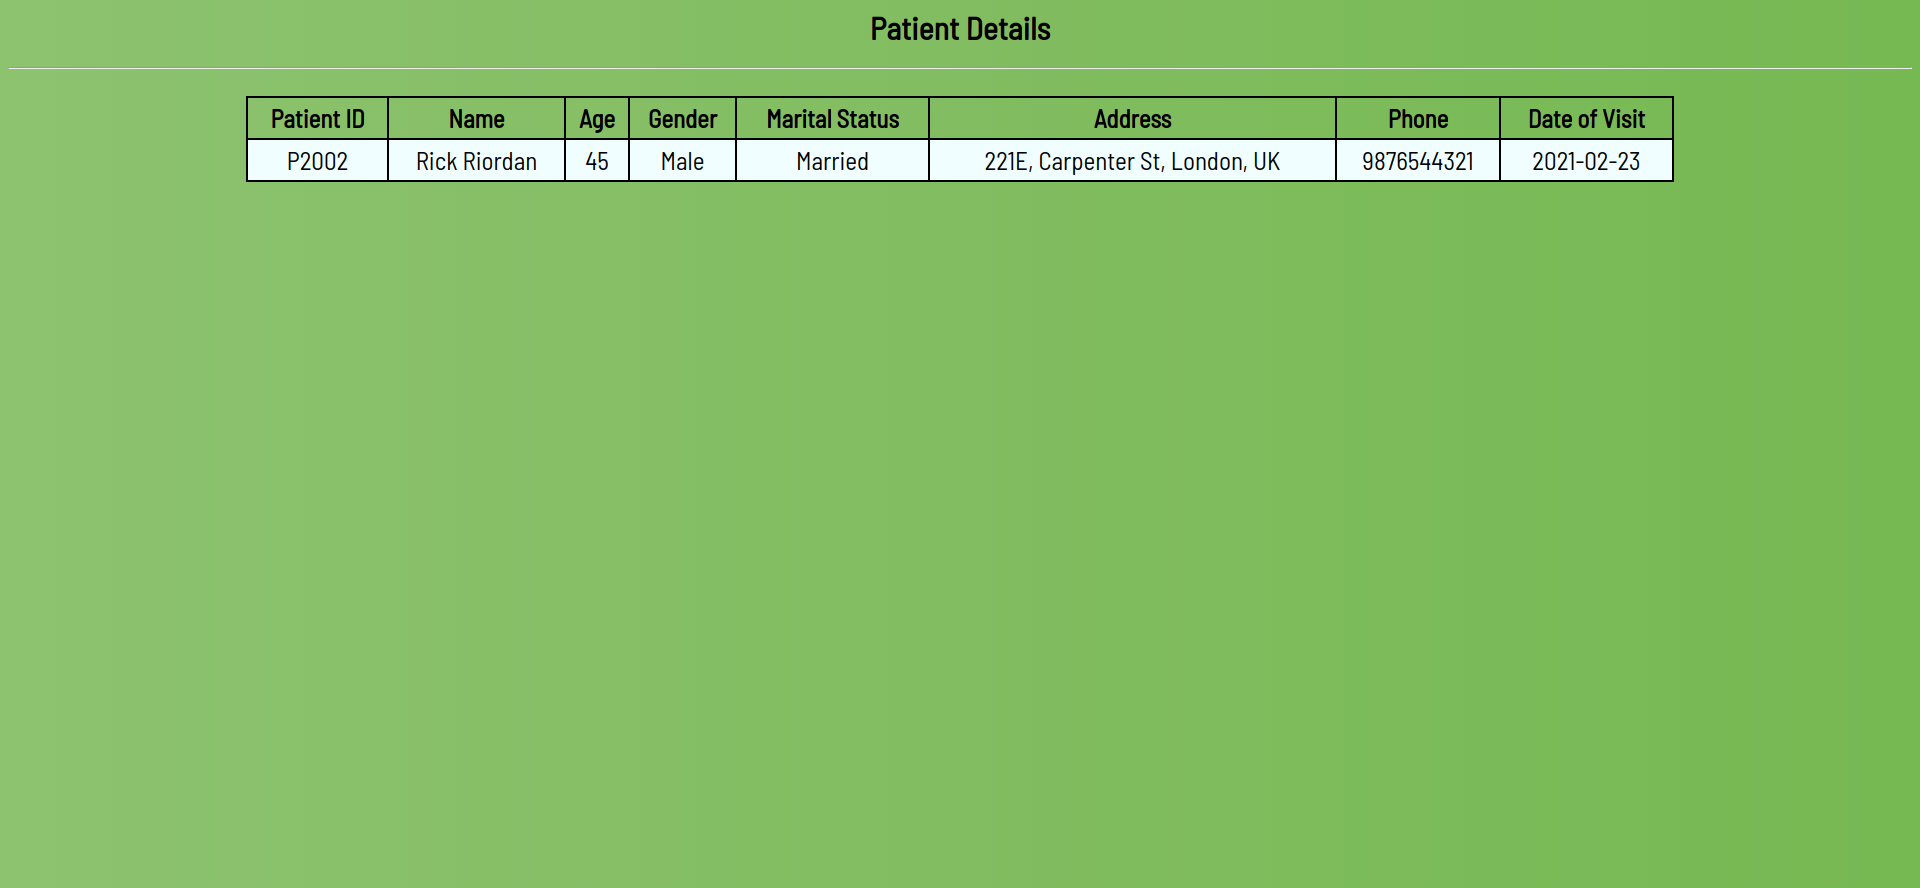
\includegraphics[height=12cm, width=16cm]{Output/PMSSearchDone.png}
\end{figure}

\newpage
\subsection*{\flushleft{Output - PMS View Page:}}
\begin{figure}[h]
\centering
\caption{Browser Output: PMS View Page.}
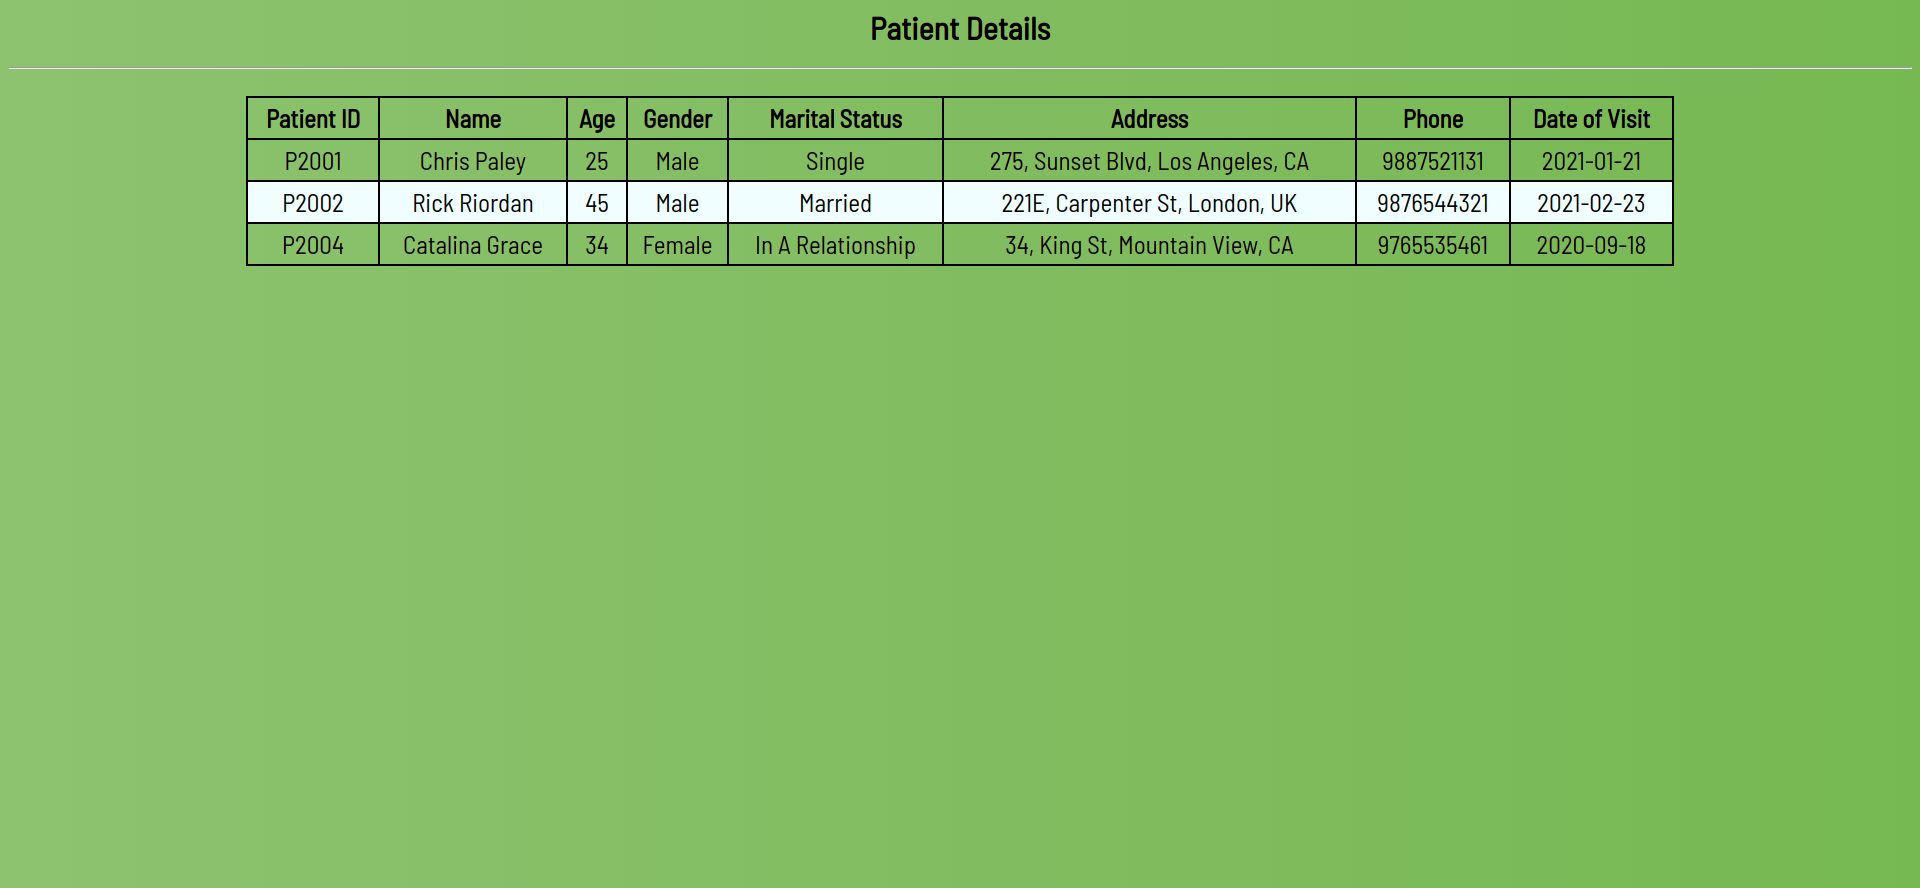
\includegraphics[height=12cm, width=16cm]{Output/PMSView4.png}
\end{figure}

\newpage
\subsection*{\flushleft{Output - SQL Table:}}
\begin{figure}[h]
\centering
\caption{Terminal Output: SQL Table.}
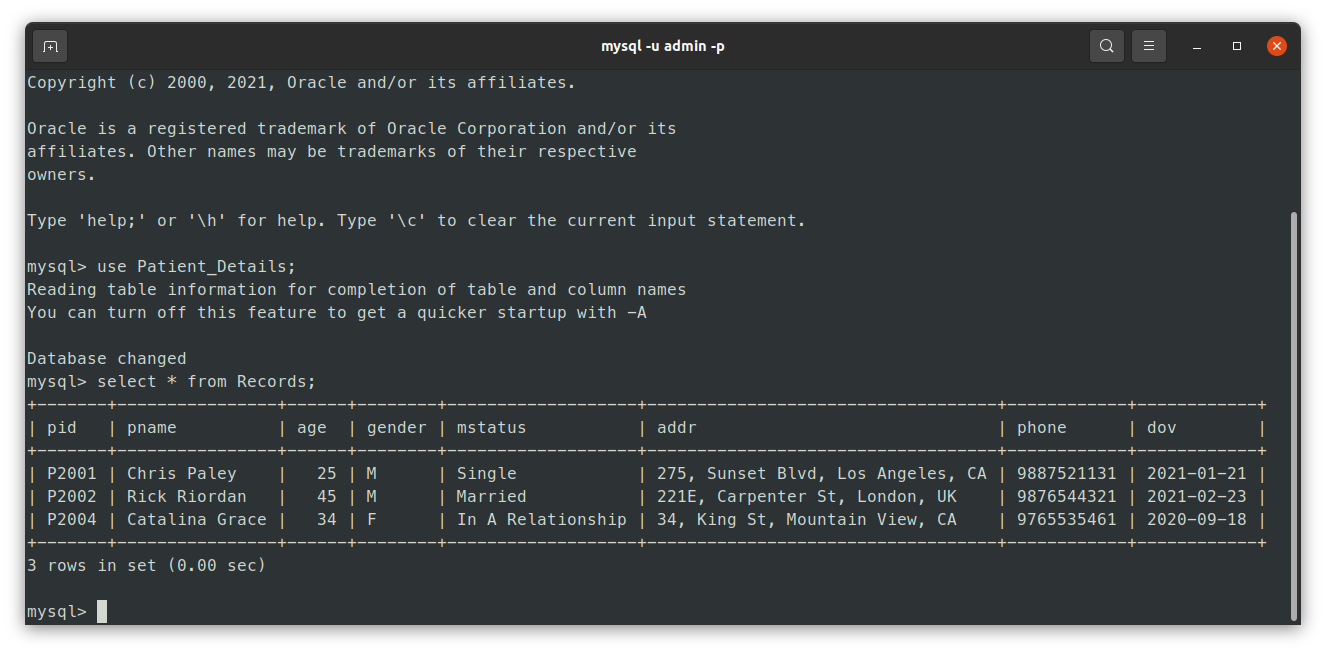
\includegraphics[height=12cm, width=18cm]{Output/SQLTable.png}
\end{figure}





%Learning Outcome
\newpage
\subsection*{\flushleft{Learning Outcome:}}
\begin{itemize}

\item From the experiment, I learnt to implement basic \textbf{Java Servlets}.
\item I learnt about the working of a Java Servlet.
\item I understood that Servlets are executed in the server-side in response to an HTML event like a submit event, and handles actions through a Request-Response mechanism.
\item I was able to serve a dynamic web page using Java Servlet programming.
\item I learnt how to extract HTML Form data from Servlets submitted using the GET query.
\item I calculated the employee's gross pay from the basic salary entered in the form in server-side using Java Servlet and displayed it back to the client-side through the browser using HTML.
\item I successfully implemented a working \textbf{Employee Registration Form} using Java Servlet programming and deployed it using the \textbf{Tomcat 9.0 Container}.
\item I refreshed my SQL concepts.
\item I learnt how to integrate MySQL to Java using JDBC Driver.
\item I was able to create a database for Patient Management using MySQL.
\item I successfully implemented JDBC connectivity to MySQL.
\item I implemented the management operations like Add, Delete, Update and Viewing Records from the client-side, and updated the back-end SQL database using Java Servlets, with the help of JDBC API calls.
\item I learnt to authorize a user with basic UserID \& Password using JavaScript. 
\item I learnt to serve an existing HTML page from a Java Servlet.
\item I understood how to handle basic SQLExceptions with the help of the try-catch block in Java.
\item I understood how to display records dynamically with the help of ResultSet Object in Java and $<$table$>$ element in HTML.
\item I was able to successfully implement a working \textbf{Patient Management System} according to the given specifications with Java Servlets and MySQL.

\end{itemize}

\end{document}
